\documentclass{beamer}
\usetheme{Frankfurt}
\usepackage{csquotes}
\usepackage{animate}
\usepackage{graphicx}

\title{History of neural networks}
\author{Yuxi Liu}
\institute{UC Berkeley}
\date{2024-08}

\begin{document}

\begin{frame}
\titlepage 
\end{frame}

\section{Prehistory}

\begin{frame}
\begin{columns}
\begin{column}{0.6\textwidth}
    \begin{displayquote}
    The thunderbolt steers all things.

    --- Heraclitus
    \end{displayquote}
\end{column}
\begin{column}{0.4\textwidth}
    \begin{figure}[t]
        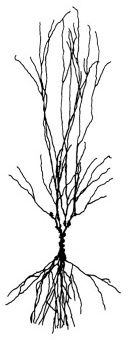
\includegraphics[width=0.6\textwidth]{figure/neuron_thunderbolt.jpg}
        \centering
    \end{figure}
\end{column}
\end{columns}
\end{frame}

\begin{frame}
\frametitle{Cajal (1900s)}
    Santiago Ramón y Cajal (1852--1934)
    \begin{itemize}
        \item Spanish neuroanatomist.
        \item Discovered neurons: the neural network is not just a network.
    \end{itemize}
    \begin{figure}[t]
        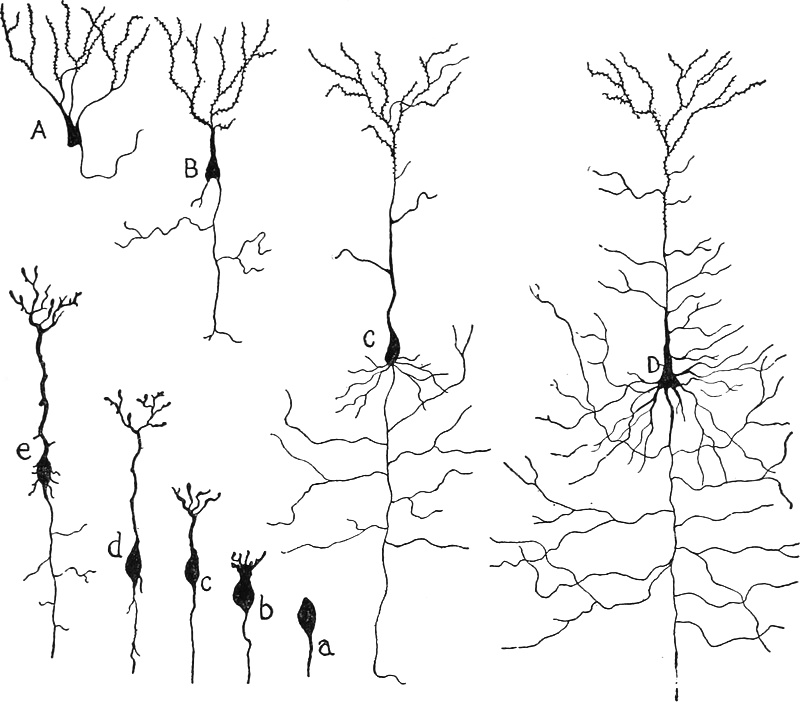
\includegraphics[width=0.7\textwidth]{figure/Cajal_neurons_examples.jpg}
        \centering
    \end{figure}
\end{frame}

\begin{frame}
    \frametitle{Cajal (1900s)}
    All neural networks are feedforward... \pause except
    \begin{figure}[t]
        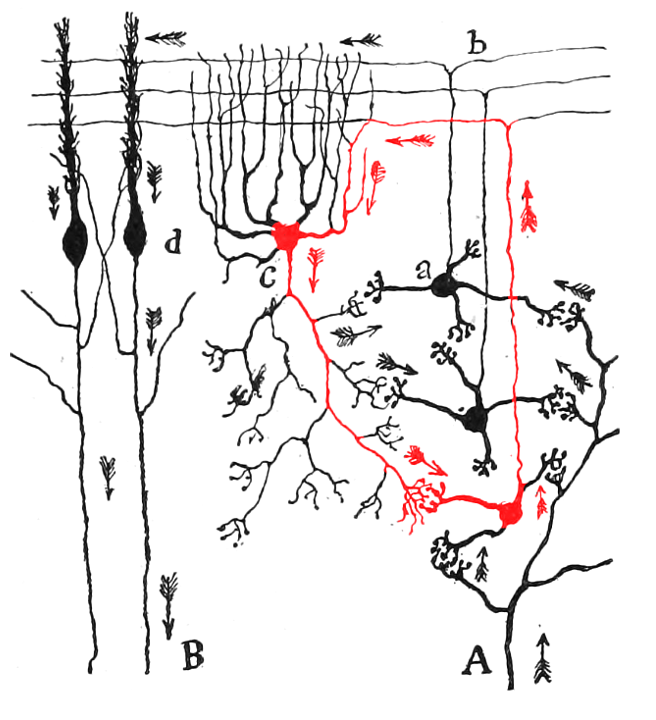
\includegraphics[width=0.5\textwidth]{figure/Cajal_RNN.png}
        \centering
        \caption{First observation of recurrent network (in the cerebellum). \cite[figure 103, page 149]{ramonycajalHistologieSystemeNerveux1909}}
    \end{figure}
    
\end{frame}

\begin{frame}
\frametitle{Vestibulo-Ocular Reflex (VOR)}
\begin{figure}[t]
    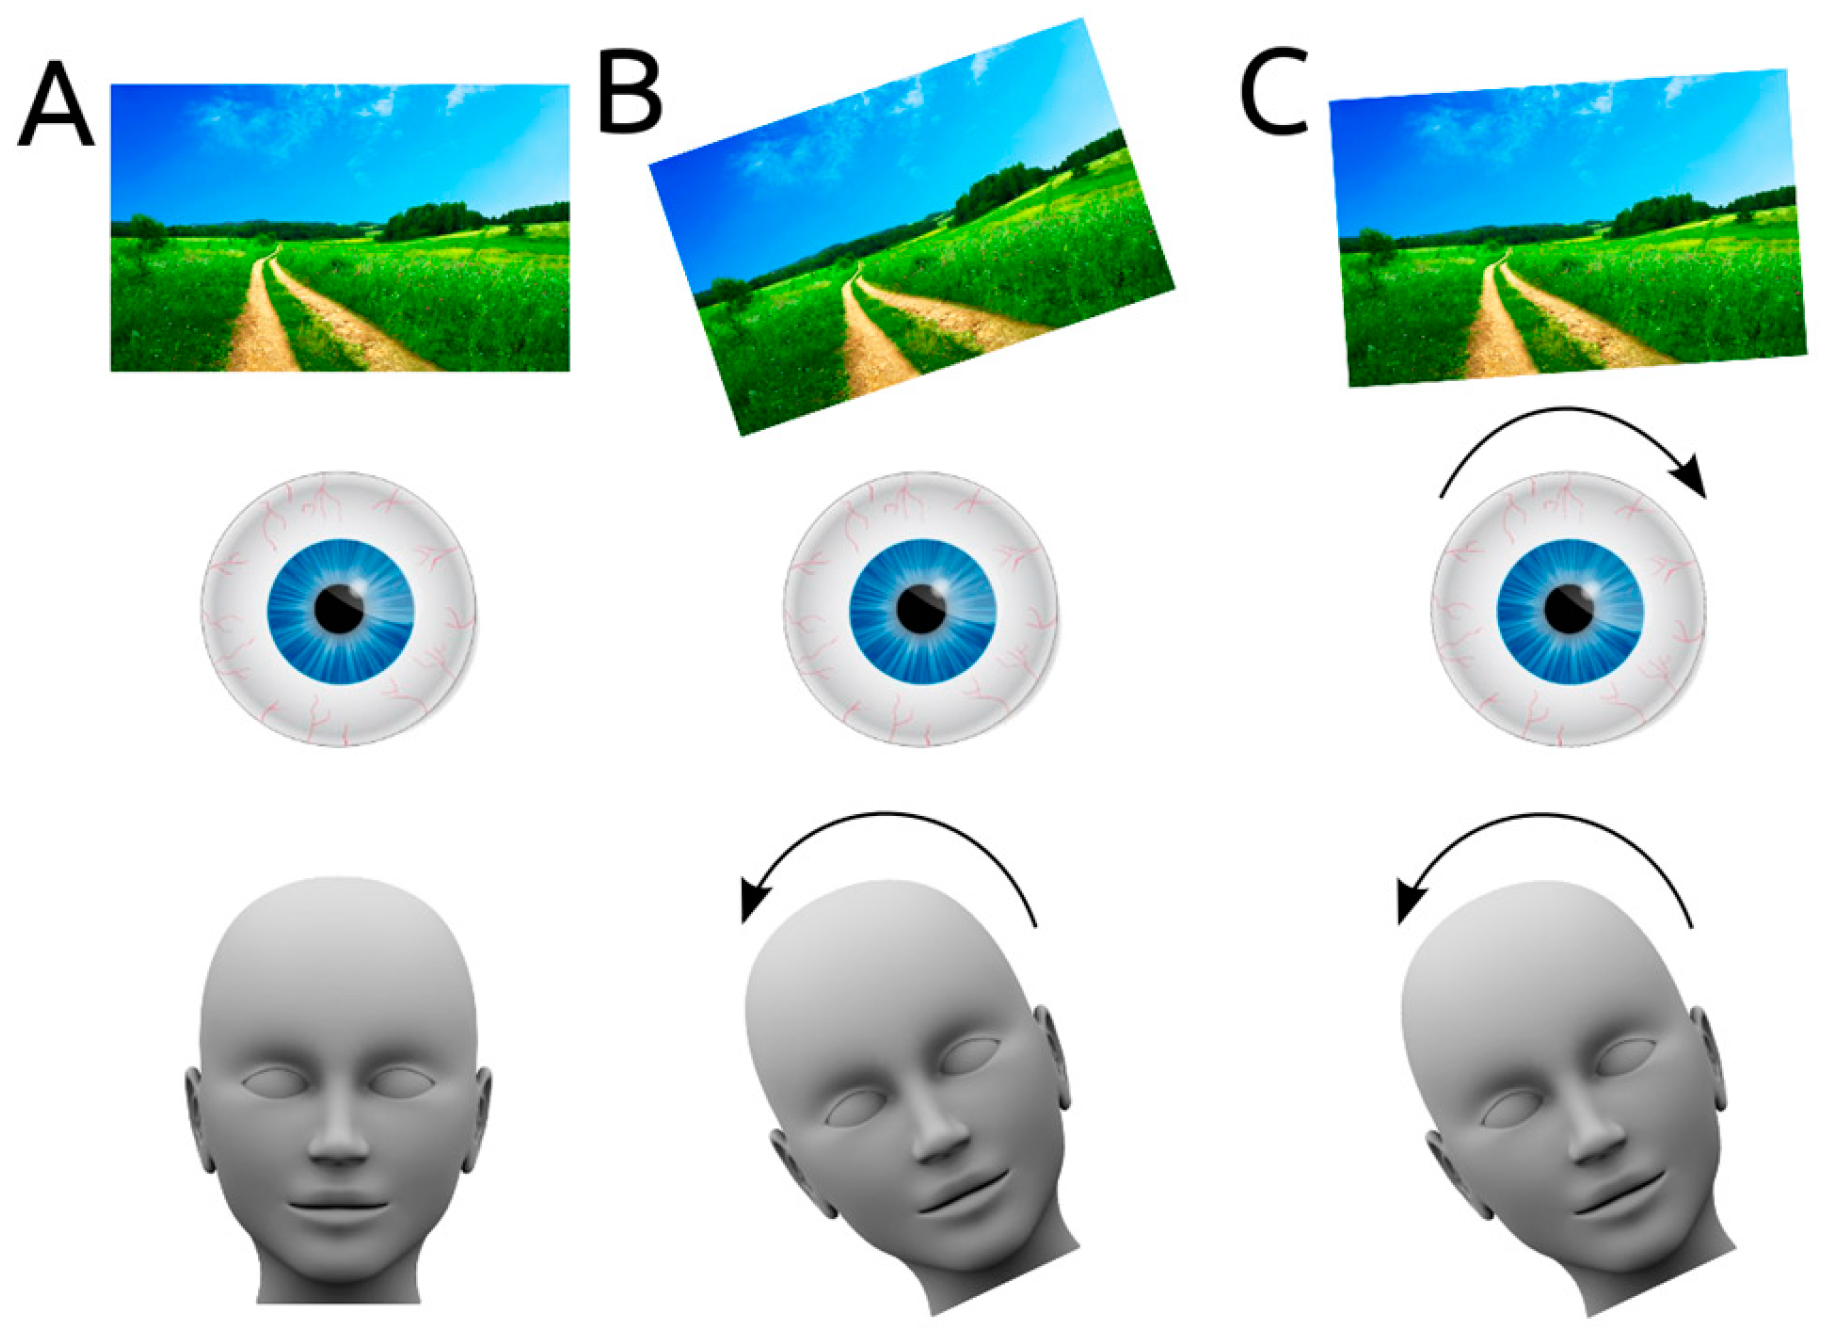
\includegraphics[width=0.8\textwidth]{figure/vestibulo-ocular_reflex.png}
    \centering
    % \caption{The VOR}
\end{figure}
\end{frame}

\begin{frame}
\frametitle{de No (1930s)}
    Rafael Lorente de Nó (1902--1990)
    \begin{itemize}
        \item Student of Cajal
        \item Discovered RNN and ResNet in the VOR.
        \item Cajal: For the sake of your career, don't publish about RNN, because nobody would believe you!...\only<2>{ so he published it after Cajal died (1934).}
    \end{itemize}

    \begin{figure}[t]
        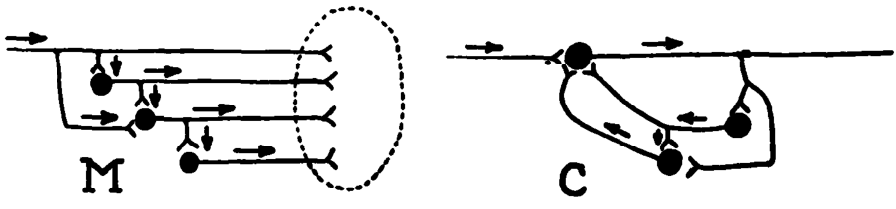
\includegraphics[width=0.8\textwidth]{figure/de_No_ResNet_RNN.png}
        \centering
        \caption{RNN and ResNet in the VOR. \cite{denoAnalysisActivityChains1938}}
    \end{figure}
    
\end{frame}

\begin{frame}
\frametitle{Hebb (1949)}
\begin{itemize}
    \item Donald O. Hebb (1904--1985)
    \item Hebbian learning: "fire together, wire together"
    \item "Reverberation" in sub-networks
\end{itemize}
\begin{figure}[t]
    \animategraphics[loop,controls,width=0.4\linewidth]{10}{figure/Hebb_RNN/Hebb_RNN-}{0}{14}
    \centering
    \caption{\cite{hebbOrganizationBehaviorNeuropsychological2002}}
\end{figure}

\end{frame}

\section{Cybernetics}

\begin{frame}
\begin{figure}[t]
    \centerline{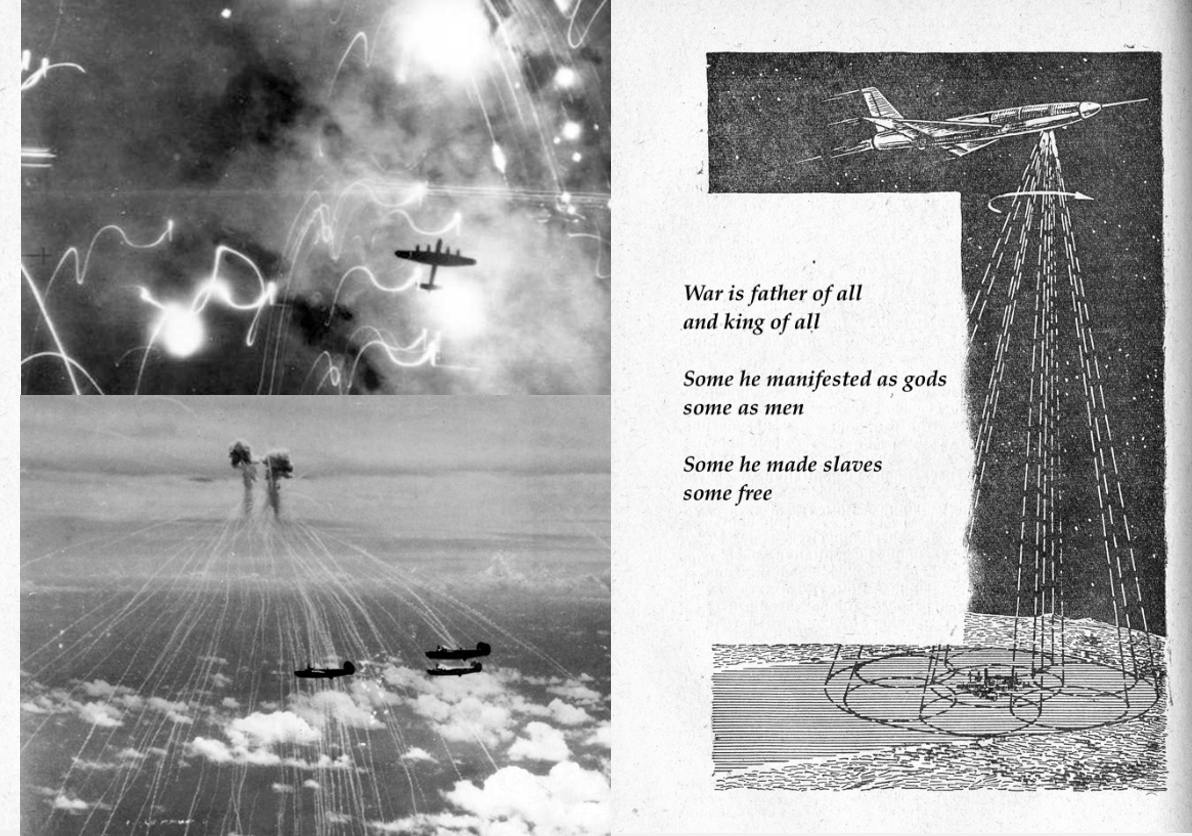
\includegraphics[width=1.2\textwidth]{figure/war_is_the_father_of_all.png}}
\end{figure}
\end{frame}

\begin{frame}
\frametitle{Fire control}
\begin{figure}[t]
    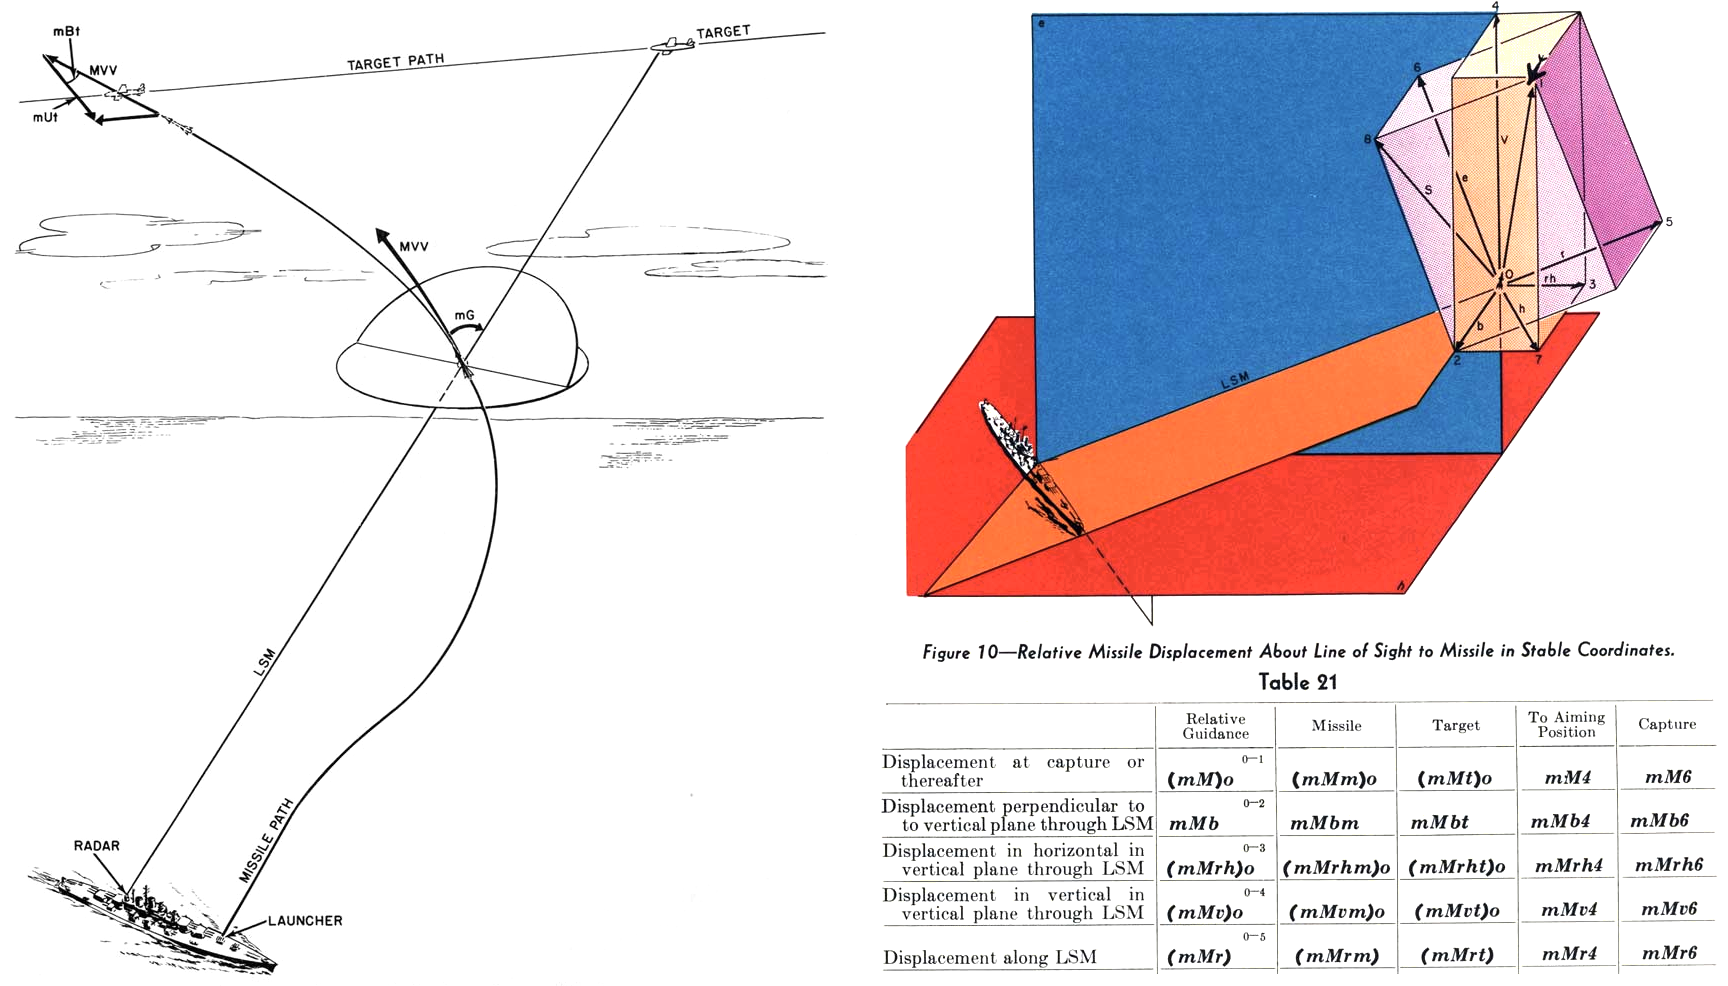
\includegraphics[width=\textwidth]{figure/fire_control_linear_regression.png}
    \centering
    \caption{Fire control as linear regression}
\end{figure}
\end{frame}

\begin{frame}
    \frametitle{Fire control}
    \begin{figure}[t]
        \includegraphics<1>[width=0.8\textwidth]{figure/war_curve_Moscow_1.jpg}
        \includegraphics<2>[width=0.8\textwidth]{figure/war_curve_Moscow_2.png}
        \centering
        \caption{Fire control as \only<2>{kernelized }linear regression}
    \end{figure}
\end{frame}
    
\begin{frame}
    \frametitle{Norbert Wiener (1941)}
    \begin{itemize}
        \item Antiaircraft fire as negative feedback control
        \item $$\mathrm{Loss} = \int \|\vec x_{\text{aircraft}}(t) - \vec x_{\text{bullet}}(t)\|^2 dt$$
        \item Minimize loss by kernelized least squares.
        \item Kernel estimated statistically from pilot data and gunner data.
    \end{itemize}
    \begin{displayquote}
        It is necessary to assimilate the different parts of the system to a single basis, either human or mechanical. Since our understanding of the mechanical elements of gun pointing appeared to us to be far ahead of our psychological understanding, we chose to try to find a mechanical analogue of the gun pointer and the airplane pilot.
    
        --- \cite[page 407]{wienerNorbertWienerLife2017}
    \end{displayquote}
    
\end{frame}

\begin{frame}
\frametitle{Norbert Wiener (1941)}
\begin{itemize}
    \item Aircraft prediction as noisy communication
    \item Past trajectory of the aircraft is a noisy channel for the future trajectory.
    \item Minimize mean-squared error by Wiener filtering
    \item Communication = Control
\end{itemize}
\begin{displayquote}
    This book represents an attempt to unite the theory and practice of two fields of work which are of vital importance in the present emergency... of time series in statistics and of communication engineering.

    --- \cite[page 1]{norbertwienerExtrapolationInterpolationSmoothing1966}
\end{displayquote}

\end{frame}

\begin{frame}
    
\frametitle{Bonus: scaling law}
\begin{columns}
\begin{column}{0.3\textwidth}
\begin{itemize}
    \item Scaling curve of B-29 at the Boeing Wichita.
    \item Scaling curves for LLM. \cite{kaplanScalingLawsNeural2020}
\end{itemize}
\end{column}
\begin{column}{0.7\textwidth}
    \begin{figure}[t]
        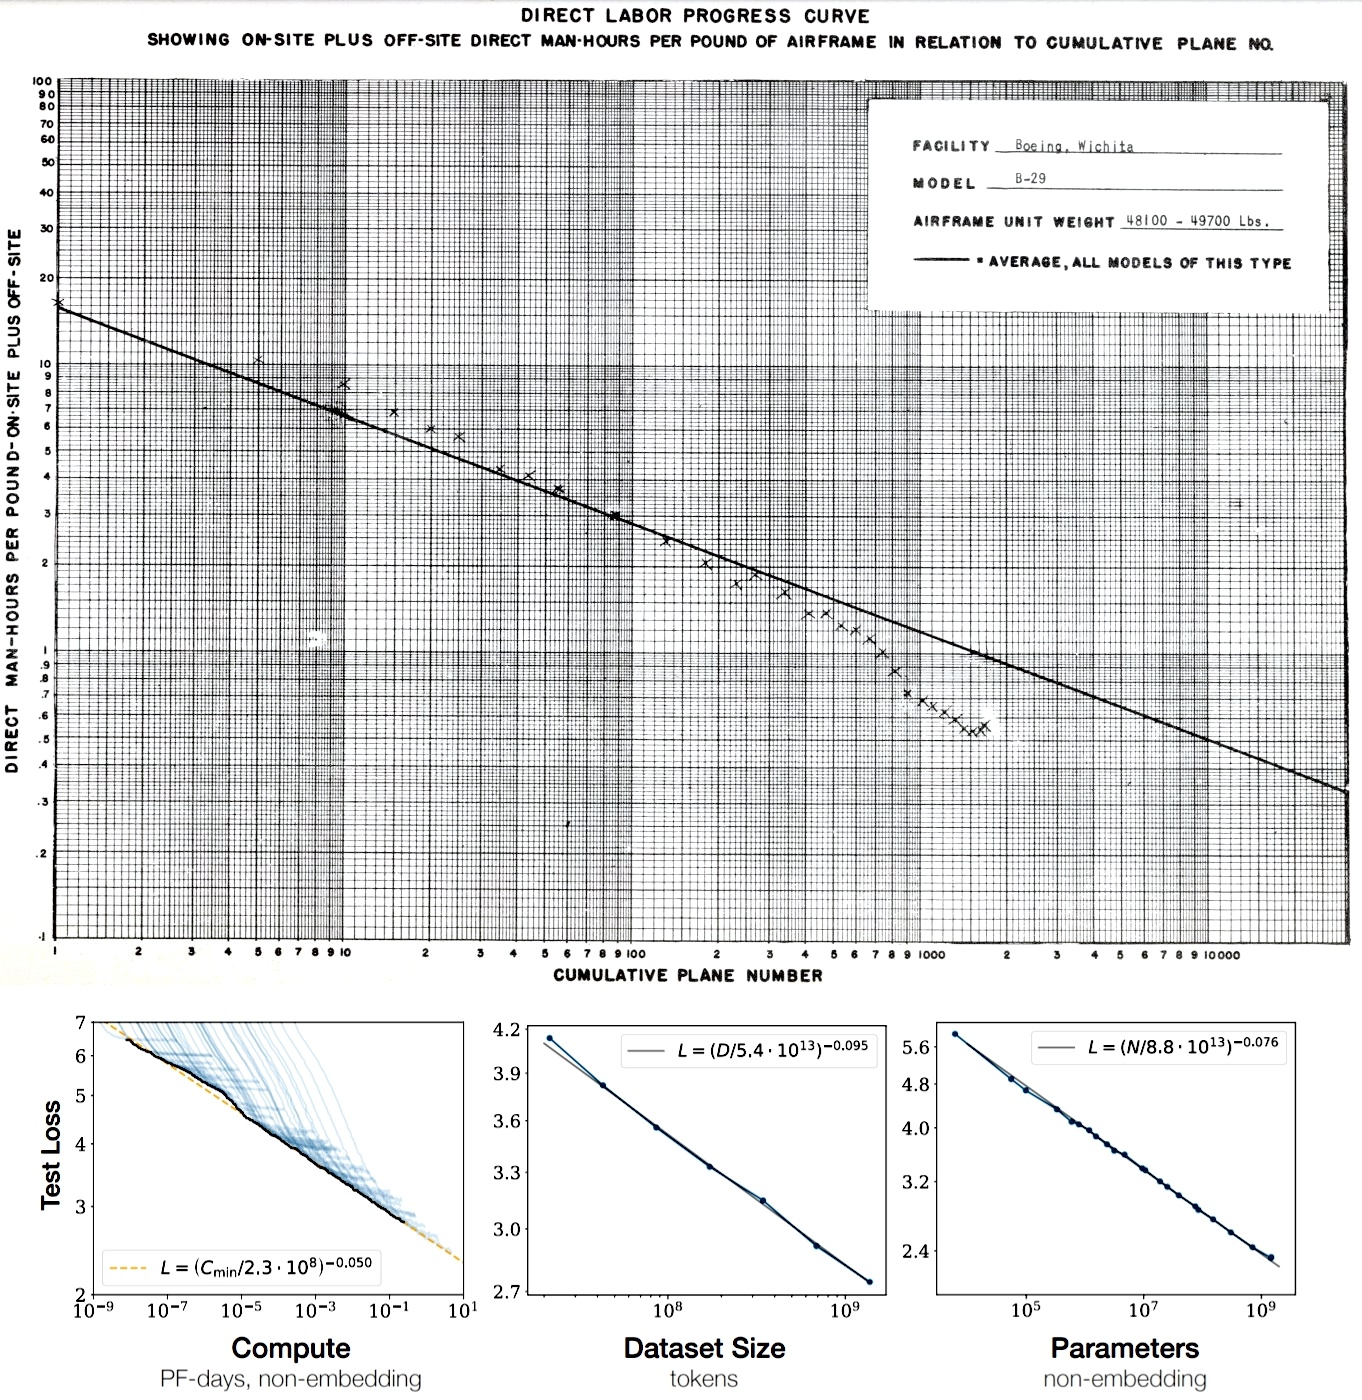
\includegraphics[width=\textwidth]{figure/bonus_scaling_plot_then_and_now.jpg}
        \centering
    \end{figure}
\end{column}
\end{columns}
\end{frame}

\begin{frame}
\frametitle{Bonus: piecewise linear regression}
\begin{figure}[t]
    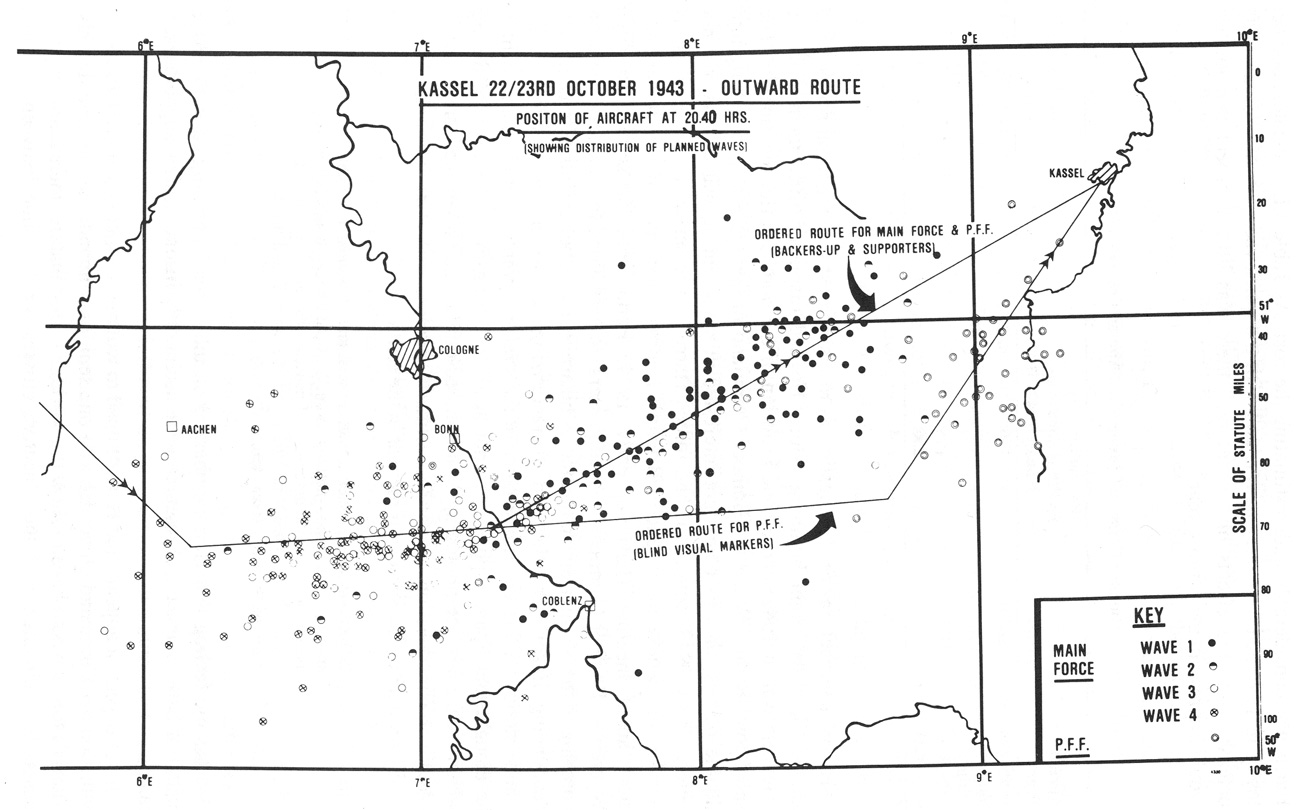
\includegraphics[width=\textwidth]{figure/Kassel_piecewise_linear.jpg}
    \centering
    \caption{Kassel bombing raid.}
\end{figure}
\end{frame}

\begin{frame}
    \frametitle{Bonus: Fire control VOR}
    
    \begin{figure}[t]
        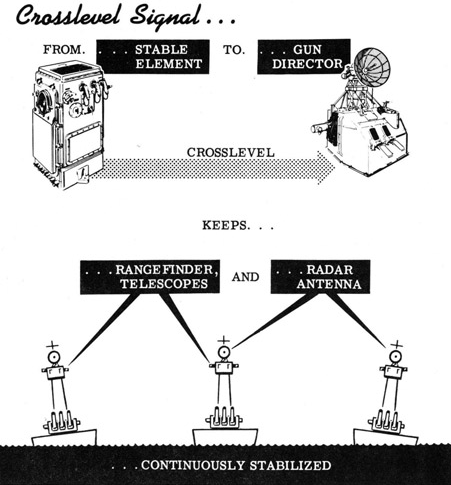
\includegraphics[width=0.6\textwidth]{figure/fire_control_VOR.png}
        \centering
        \caption{Fire control with vestibulo-ocular reflex}
    \end{figure}
\end{frame}
    
\begin{frame}
\frametitle{McCulloch \& Pitts (1943)}
\begin{itemize}
    \item Warren McCulloch (1898--1969): neuro-philosopher.
    \item Walter Pitts (1923--1969): tragic logician.
    \item Met in 1941. Started working on a mathematical theory of thinking.
    \item Inspired by cybernetics, causal loops, memory, learning, neural logic, hallucination, epilepsy...
    \item Went to the Macy conferences. (de No was there too)
    \item \cite{mccullochLogicalCalculusIdeas1943}: Proposed artificial neural network.
\end{itemize}
\begin{displayquote}
    What is a number, that a man may know it, and a man, that he may know a number?

    --- Warren McCulloch
\end{displayquote}

\end{frame}

\begin{frame}
\frametitle{McCulloch \& Pitts (1943)}
\begin{itemize}
    \item Universality: Any boolean function is computed by some feedforward network.
    \item Feedforward network with Hebbian learning is equivalent to a recurrent network without Hebbian learning.
\end{itemize}

\begin{columns}
\begin{column}{0.5\textwidth}
\begin{figure}[t]
    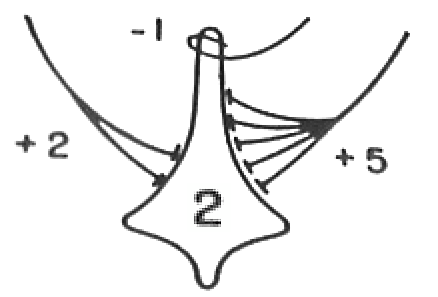
\includegraphics[width=0.6\textwidth]{figure/MP_neuron.png}
    \centering
    \caption{A single MP neuron.}
\end{figure}
\end{column}
\begin{column}{0.5\textwidth}
    \begin{figure}[t]
        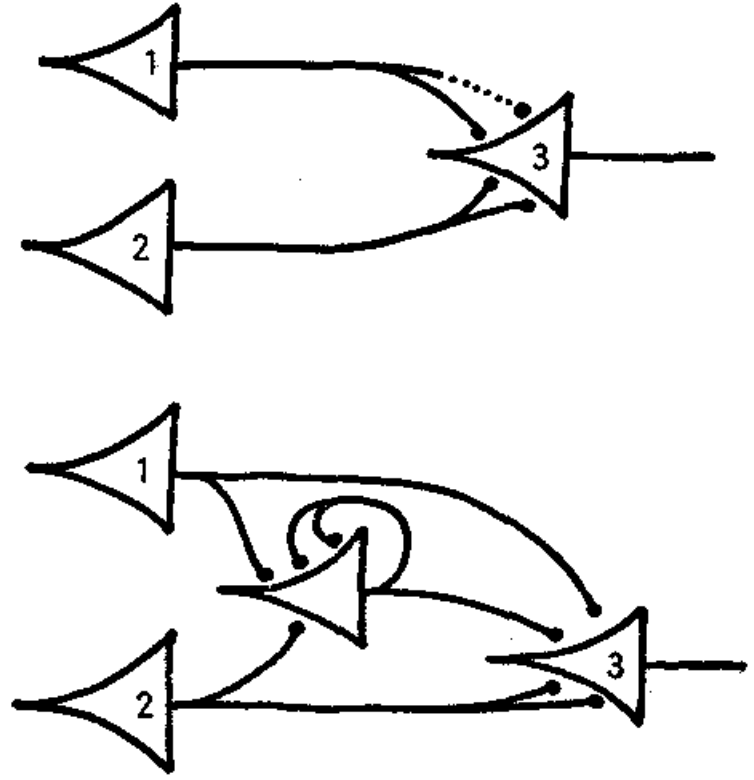
\includegraphics[width=0.6\textwidth]{figure/MP_recurrent_learning.png}
        \centering
        \caption{Hebbian learning is equivalent to recurrence.}
    \end{figure}        
\end{column}
\end{columns}

\end{frame}

\begin{frame}
    \frametitle{Why was causal loop unacceptable?}
    I have no firm answers, but I have some ideas...

    \begin{itemize}
        \item Reflexes are simpler to study for neuroscientists.
        \item Feedback is much harder to solve mathematically.
        \item Loops threaten linear causality: $\text{cause}\to\text{effect}$.
        \item Dominance of personalities: Cajal, Pavlov, Skinner...
    \end{itemize}
\end{frame}

\begin{frame}
    \frametitle{Comment: Progress is possible}
    \begin{itemize}
        \item Early 20th century, the brain was often analogized to a telephone switchboard
        \item Now, analogized to a neural network
        \item Some commentators sneer that our analogy is nothing but techno-fashion
        \item But telephone switchboards are feedforward, while neural network have feedback.
        \item Lesson: There is progress!
    \end{itemize}
    \begin{figure}[t]
        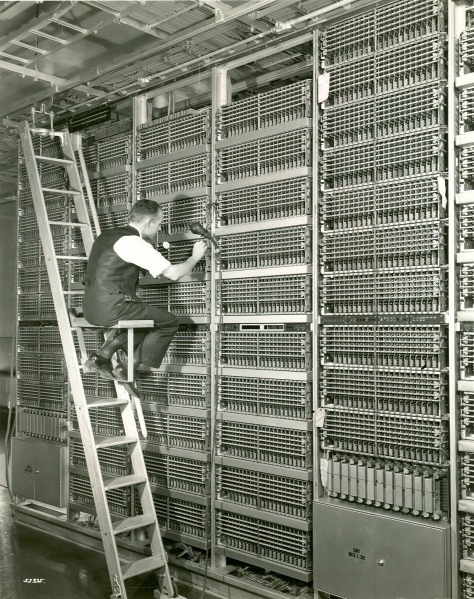
\includegraphics[width=0.4\textwidth]{figure/Crossbar_NY_1938-05.jpg}
        \centering
        \caption{Crossbar switching at a New York telephone exchange center (1938).}
    \end{figure}
    
\end{frame}

\section{Perceptron era (50s--60s)}

\begin{frame}
\frametitle{1950s neural networks}
Multiple neural networks in the early 1950s. Most notable is Minsky's SNARC (1952): maze-running rat with 40 neurons, trained by reinforcement Hebbian learning. Every time the operator presses a reward button, the synaptic strengths change by Hebbian learning.

\begin{columns}
    \begin{column}{0.5\textwidth}
    \begin{figure}[t]
        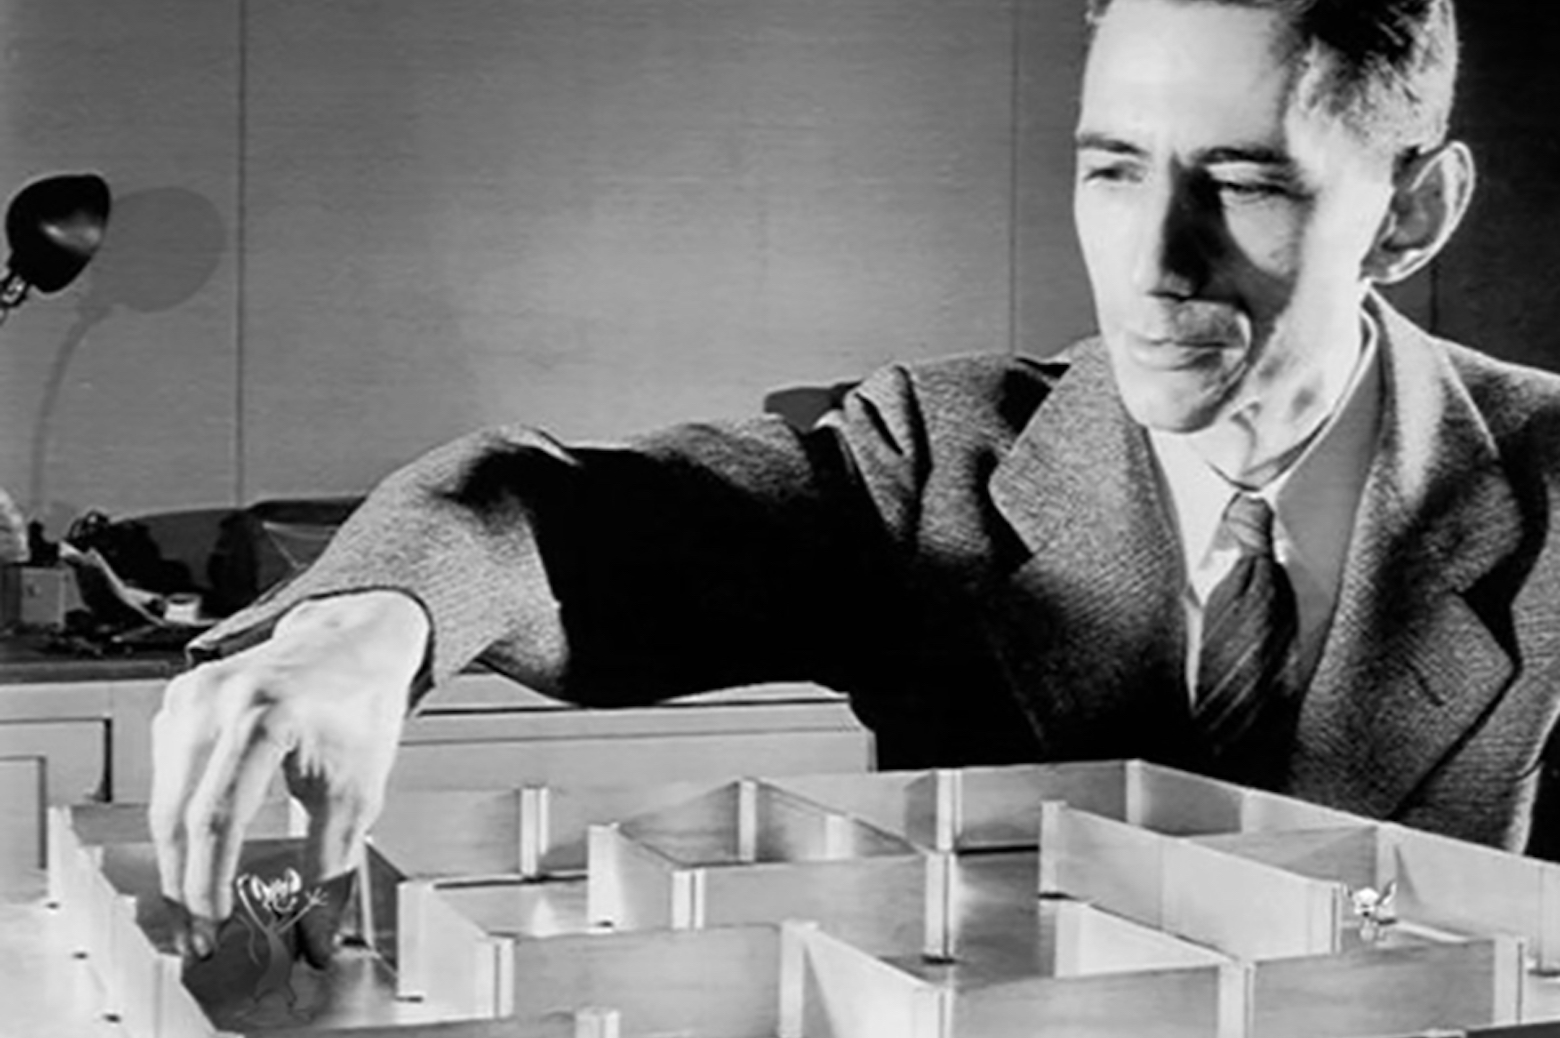
\includegraphics[width=\textwidth]{figure/Shannon_mouse_robot.jpg}
        \centering
        \caption{Shannon and his robot mouse.}
    \end{figure}
    \end{column}
    \begin{column}{0.5\textwidth}
        \begin{figure}[t]
            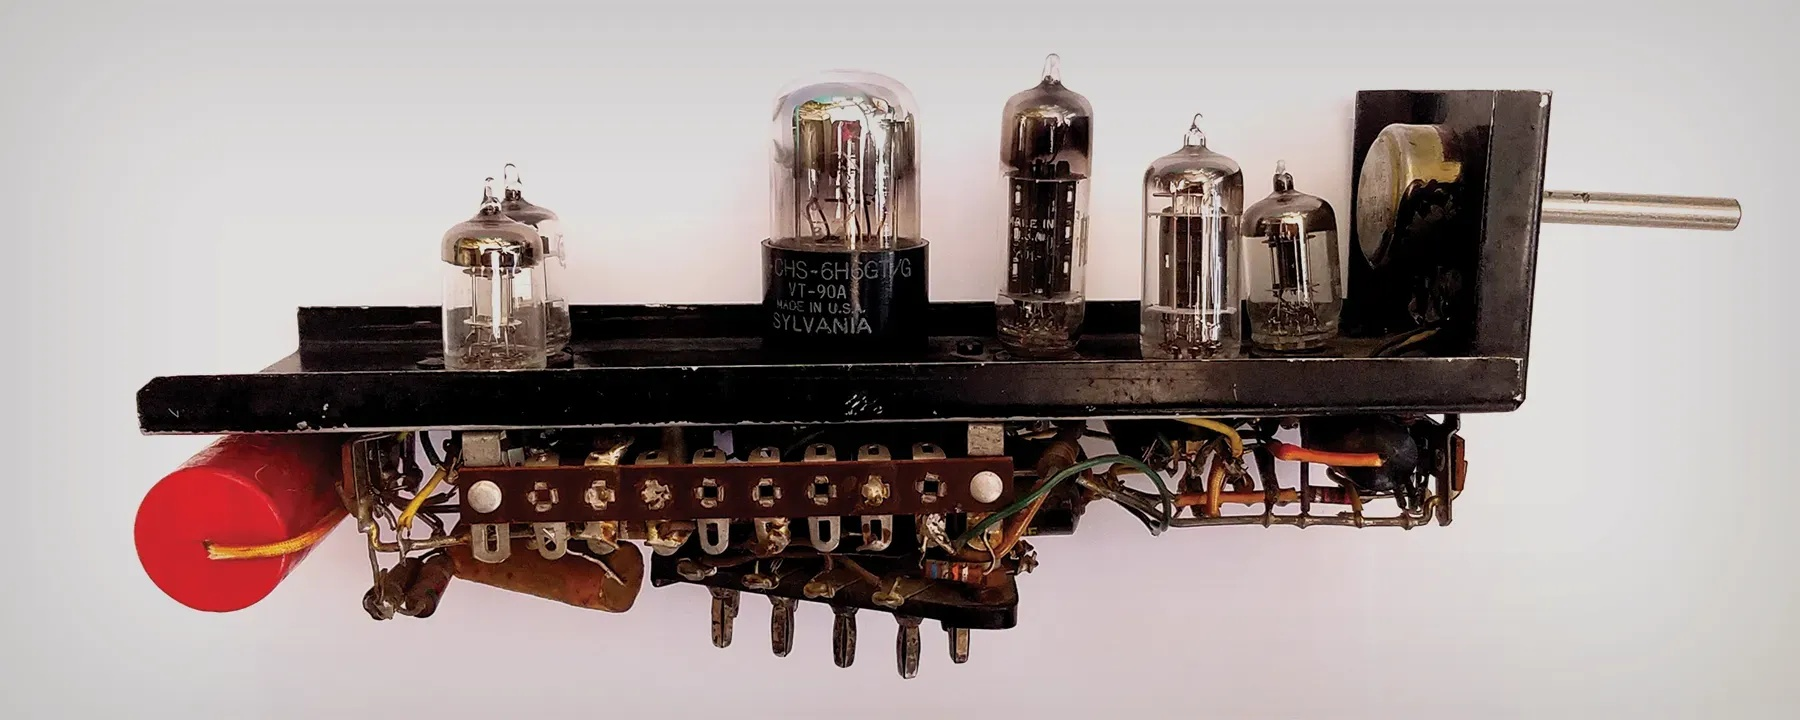
\includegraphics[width=\textwidth]{figure/SNARC_neuron.jpg}
            \centering
            \caption{A SNARC neuron.}
        \end{figure}        
    \end{column}
\end{columns}
\end{frame}

\begin{frame}
\frametitle{Perceptron}
\begin{itemize}
    \item Frank Rosenblatt (1928--1971): Did most of his work during 1957--1964.
    \item \cite{rosenblattPerceptronProbabilisticModel1958} and \cite{rosenblattPrinciplesNeurodynamicsPerceptrons1962}: multilayered perceptrons.
    \item A perceptron is a binary neuron: $\theta(\sum_i w_ix_i + b)$, where $\theta$ is the 0-1 activation function.
\end{itemize}
\begin{figure}[t]
    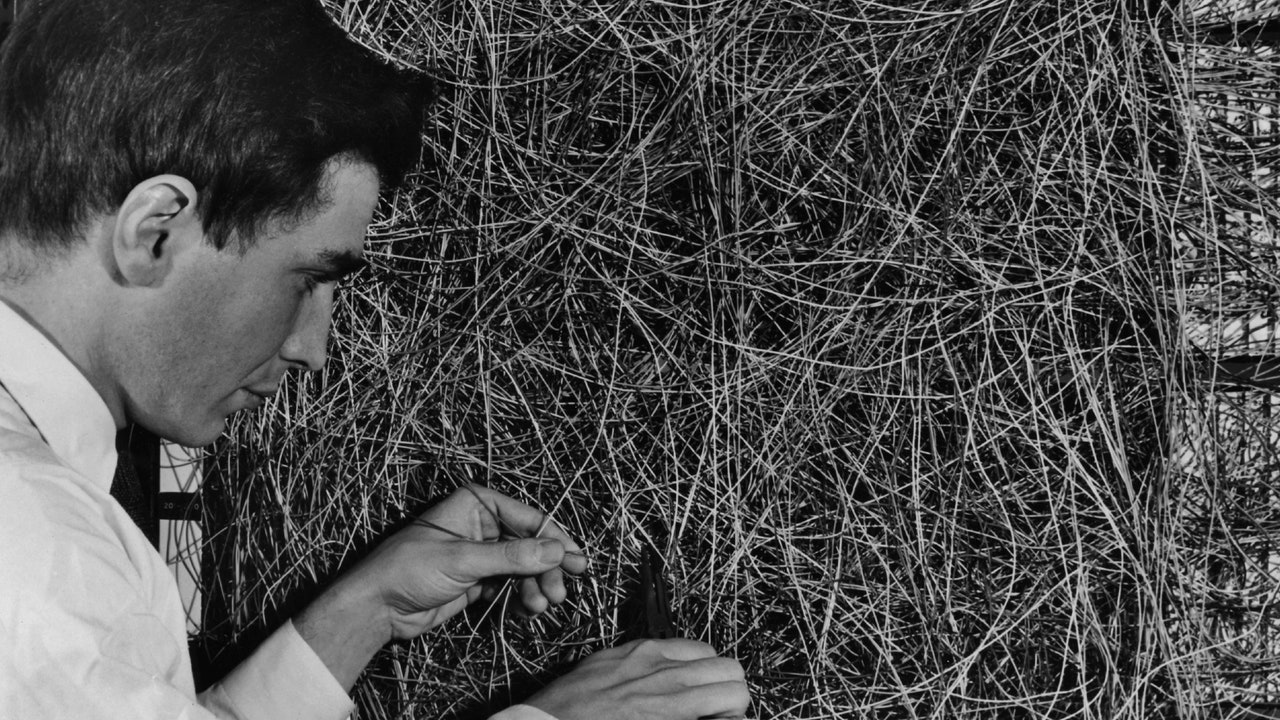
\includegraphics[width=\textwidth]{figure/Rosenblatt_perceptron_wiring.jpeg}
    \centering
    \caption{The Perceptron Mark I (1958).}
\end{figure} 
\end{frame}

\begin{frame}
    \frametitle{Example}
    \begin{itemize}
        \item First layer fixed.
        \item Second layer has both residual connection and learned connection. The learned weights increase by Hebbian learning, and decay exponentially.
        \item Third layer by the perceptron learning rule.
    \end{itemize}
    \begin{figure}[t]
        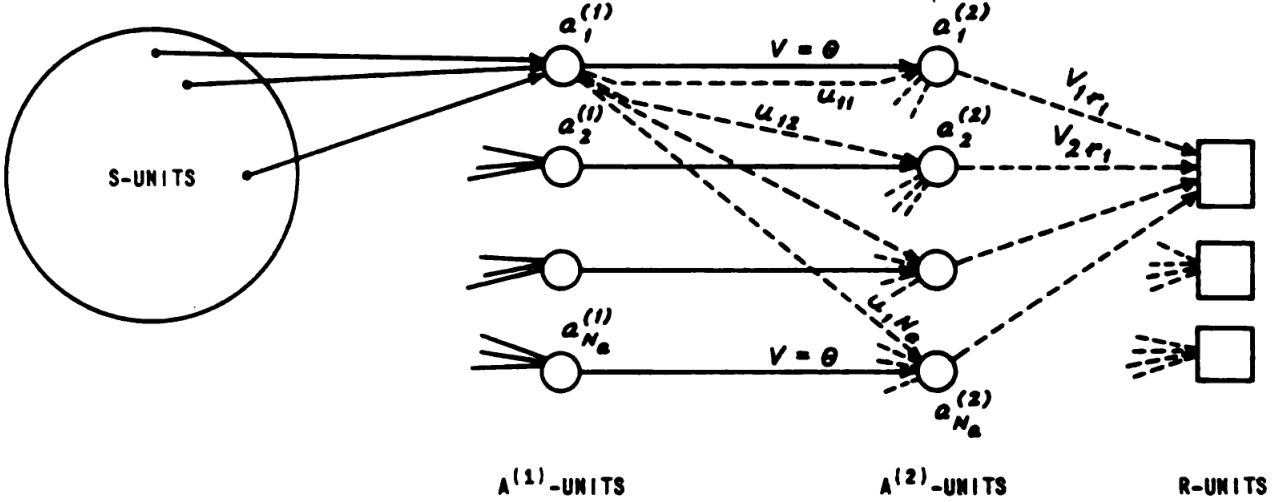
\includegraphics[width=\textwidth]{figure/rosenblatt_figure_42.png}
        \centering
        \caption{A multilayered perceptron. \cite[page 347]{rosenblattPrinciplesNeurodynamicsPerceptrons1962}}
    \end{figure}  
\end{frame}

\begin{frame}
\begin{columns}
    \begin{column}{0.5\textwidth}
    \begin{figure}[t]
        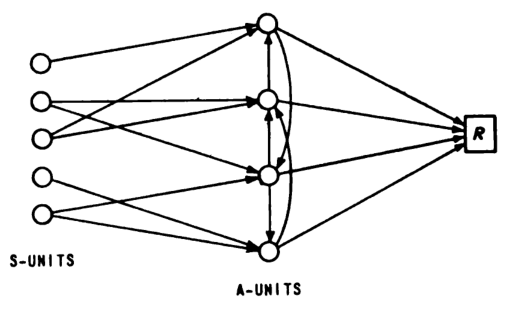
\includegraphics[width=\textwidth]{figure/Rosenlatt_Hopfield_network.png}
        \centering
        \caption{Hopfield network? (Figure 47)}
    \end{figure}
    \end{column}
    \begin{column}{0.5\textwidth}
        \begin{figure}[t]
            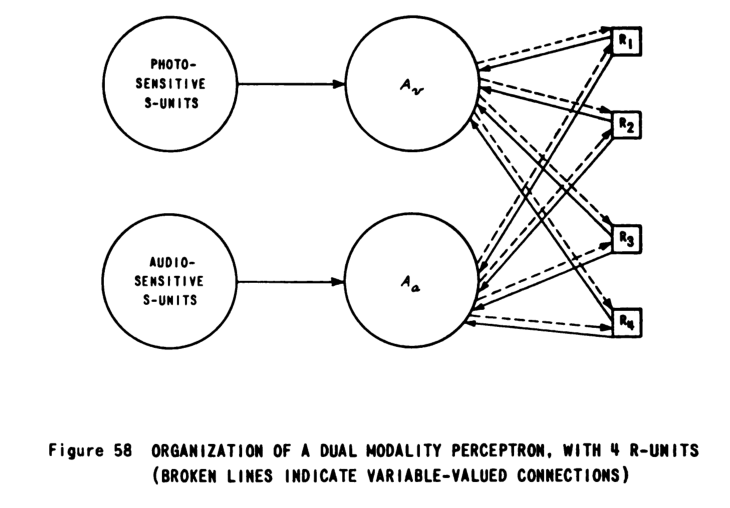
\includegraphics[width=\textwidth]{figure/Rosenblatt_multimodal.png}
            \centering
            \caption{Multimodality. (Figure 58)}
        \end{figure}
    \end{column}
\end{columns}
\end{frame}

\begin{frame}
    \frametitle{Tobermory}
    \begin{itemize}
        \item Speech recognition. Named after a talking cat.
        \item 2 hidden layers, 12,000 weights. Takes up an entire room.
        \item Built during 1961--1967. When completed, already slower than simulation on IBM machines.
    \end{itemize}
    \begin{figure}[t]
        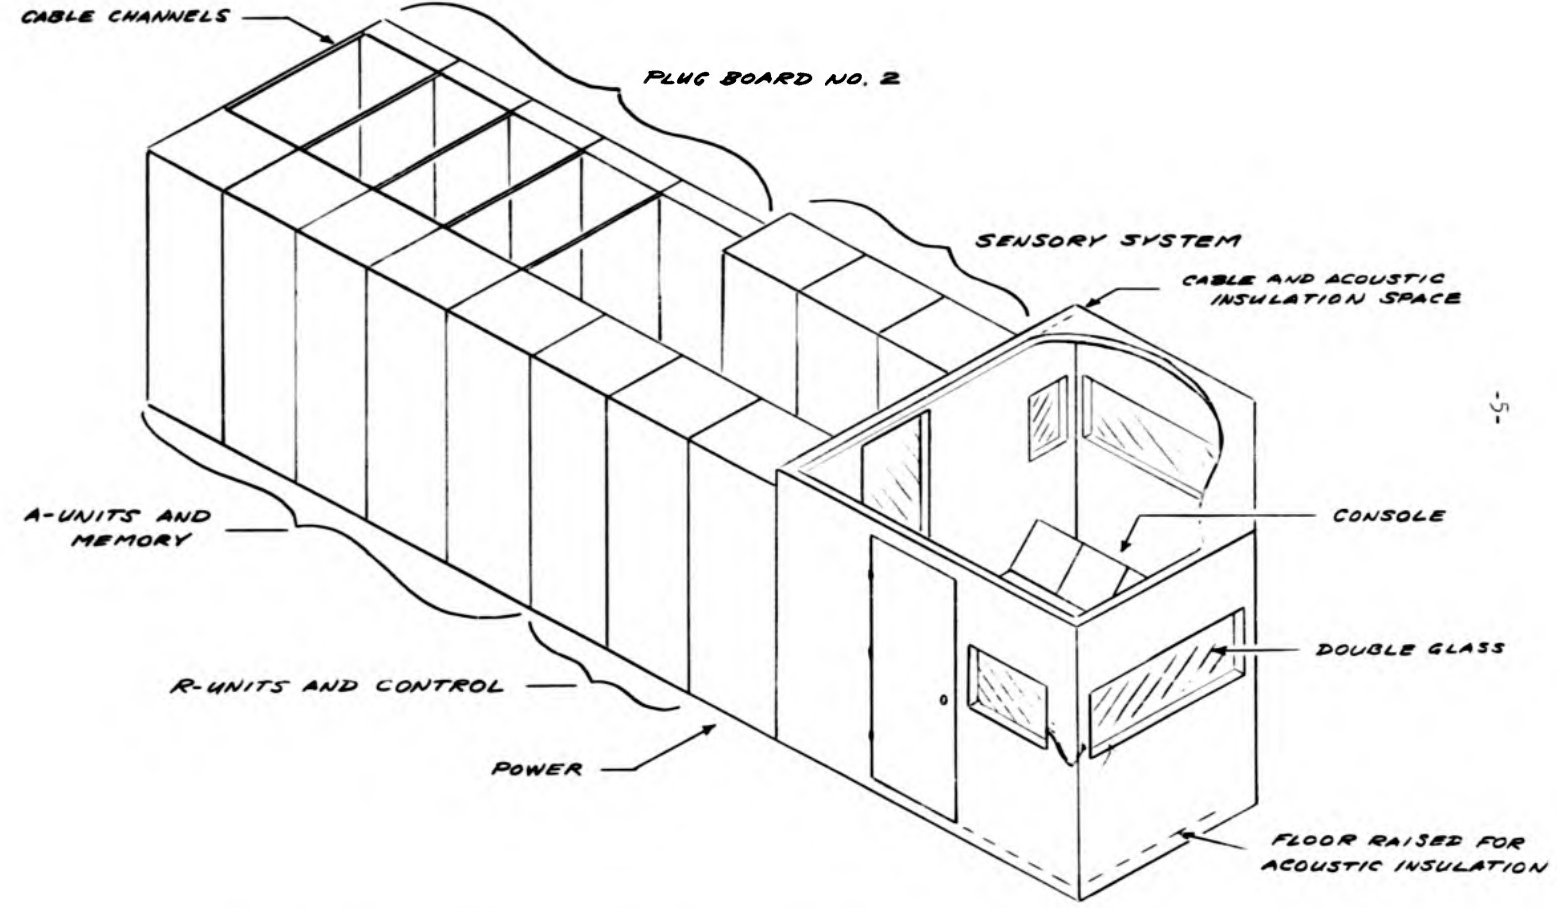
\includegraphics[width=0.7\textwidth]{figure/Tobermory.png}
        \centering
        \caption{Schematic for Tobermory.}
    \end{figure}  
\end{frame}

\begin{frame}
\frametitle{MINOS}

\begin{itemize}
    \item MINOS project (1958--1967), at Stanford Research Institute (SRI).
    \item Character recognition for military applications.
    \item MINOS II (1963): analog image $\to$ 100 binary hidden neurons by 100 optical masks, then a linear layer to 63 binary outputs by perceptron learning rule.
\end{itemize}

\begin{figure}[t]
    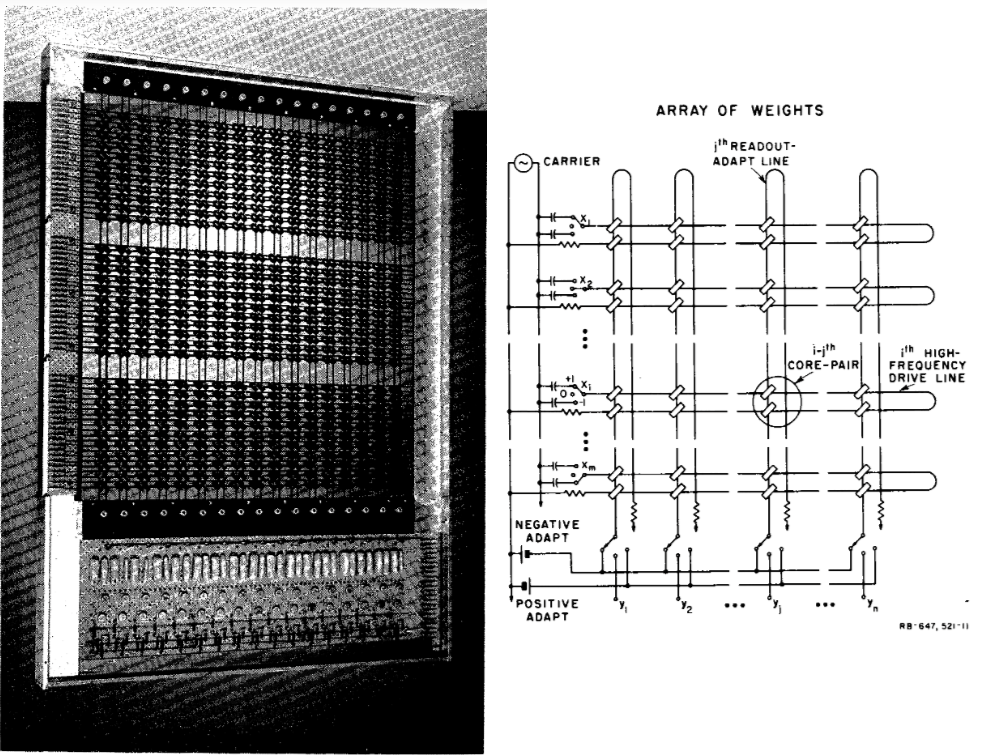
\includegraphics[width=0.5\textwidth]{figure/MINOS_II.png}
    \centering
    \caption{Weight matrix for MINOS II (1962). World's first TPU?}
\end{figure}
    
\end{frame}

\begin{frame}
\frametitle{ADALINE}
ADALINE (adaptive linear), single binary perceptron, trained by gradient descent on squared error $(\sum_i w_i x_i + b - y)^2$. Developed by Bernard Widrow's group.

\begin{figure}[t]
    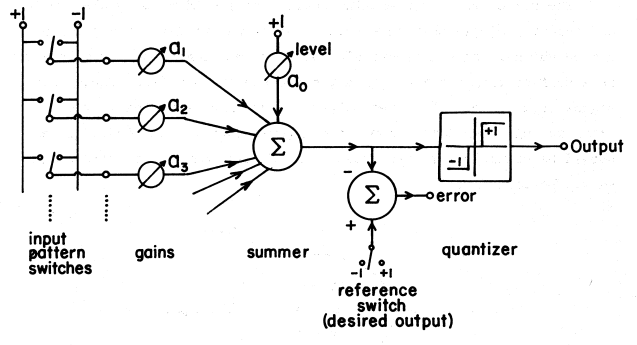
\includegraphics[width=0.6\textwidth]{figure/ADALINE_circuit.png}
    \centering
    \caption{Circuit diagram of ADALINE.}
\end{figure}

\end{frame}

\begin{frame}
\frametitle{ADALINE}
\begin{figure}[t]
    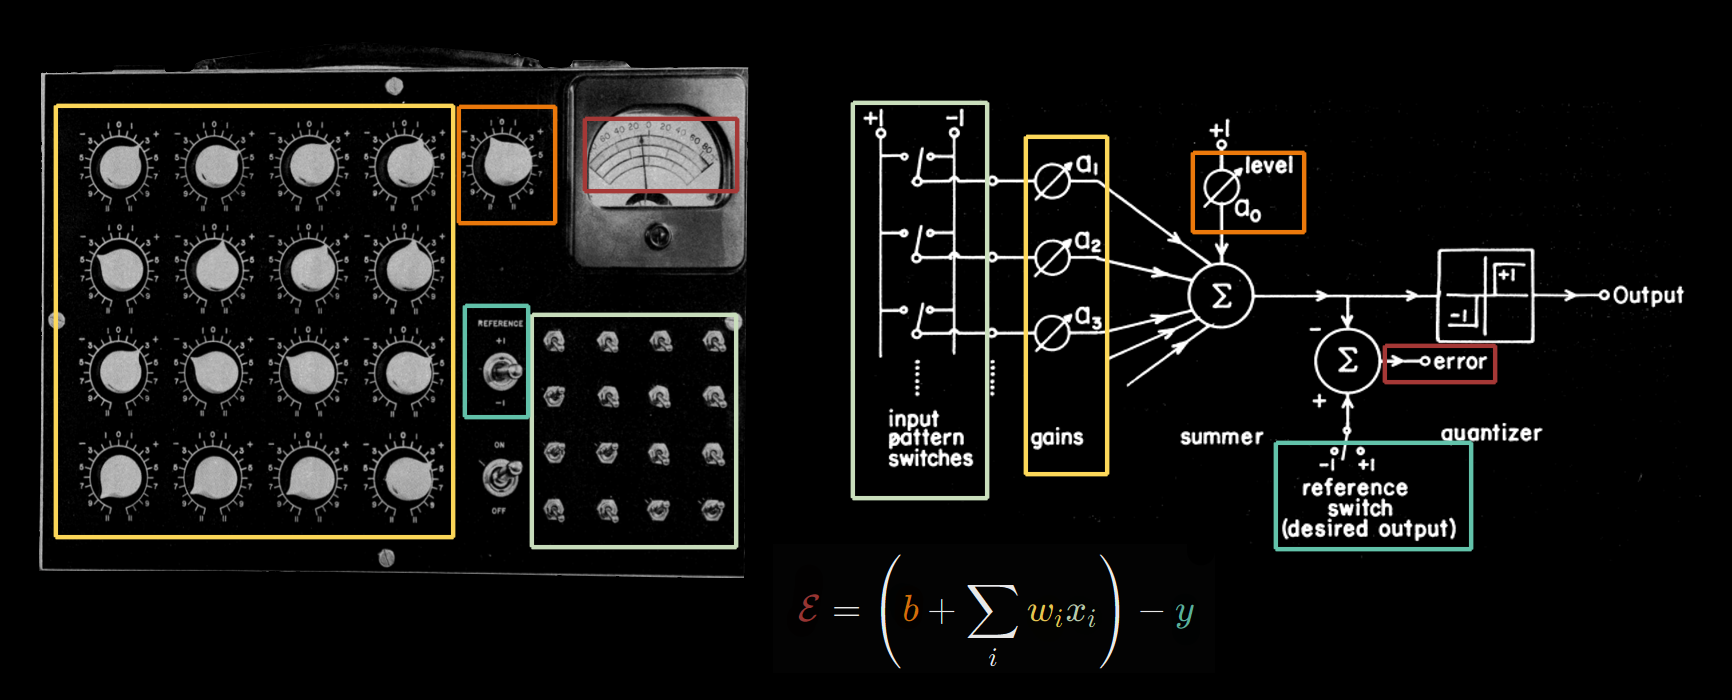
\includegraphics[width=\textwidth]{figure/ADALINE.png}
    \centering
    \caption{16 input switches and 1 output switch. Manually operated.}
\end{figure}
\end{frame}

\begin{frame}
\frametitle{ADALINE}
\begin{columns}
    \begin{column}{0.5\textwidth}
        \begin{figure}[t]
            \includegraphics[width=\textwidth]{figure/knobby_ADALINE.jpg}
            \centering
            \caption{Widrow performing brain surgery on his first-born.}
        \end{figure}
    \end{column}
    \begin{column}{0.5\textwidth}
        \begin{figure}[t]
            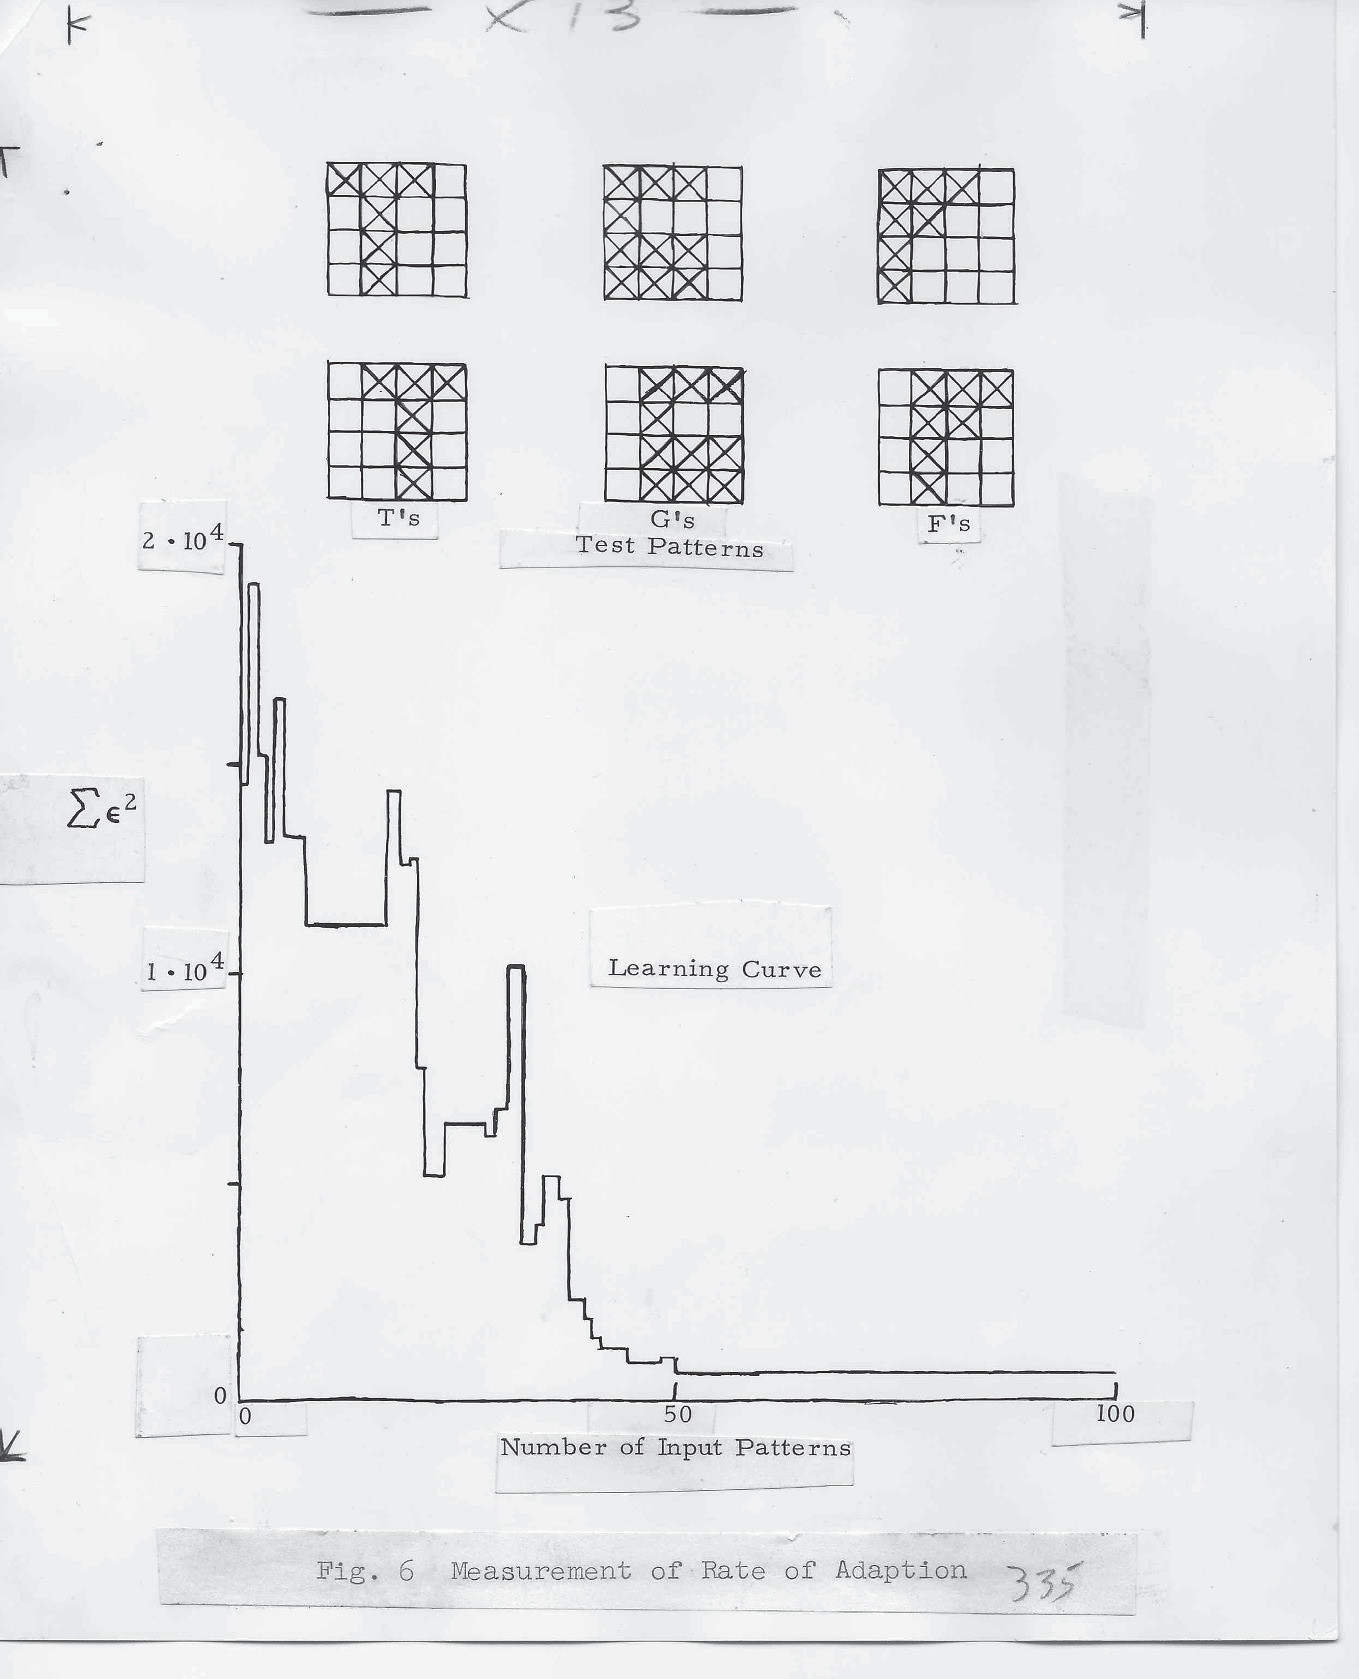
\includegraphics[width=\textwidth]{figure/ADALINE_learning_curve.png}
            \centering
            \caption{Input and learning curve.}
        \end{figure}
    \end{column}
\end{columns}
\end{frame}

\begin{frame}
\frametitle{MADALINE}
They also tried MADALINE (many ADALINE), with many hacky rules, but never gradient descent (because of the binary activation).

\begin{figure}[t]
    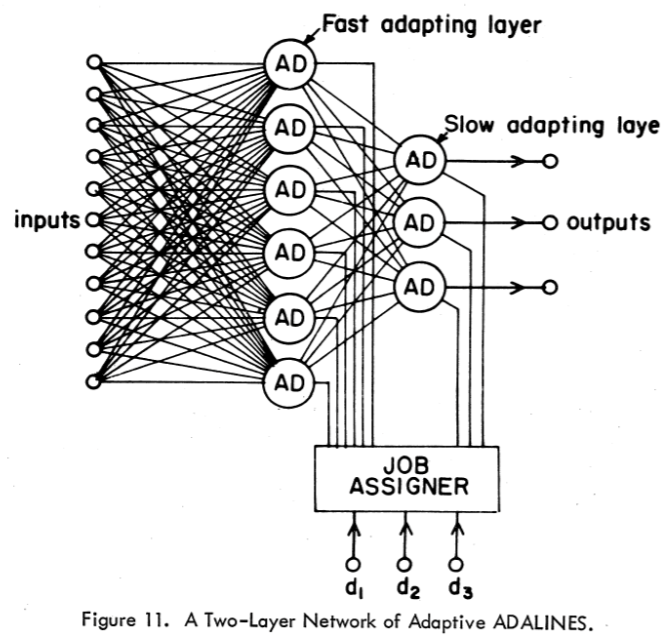
\includegraphics[width=0.5\textwidth]{figure/MADALINE.png}
    \centering
    \caption{MADALINE from 1962. The "JOB ASSIGNER" learning rule is too hacky to explain. \cite{widrowGeneralizationInformationStorage1962}}
\end{figure}
\end{frame}

\section{Winter (60s--70s)}

\begin{frame}
    
    \begin{figure}[t]
        \centerline{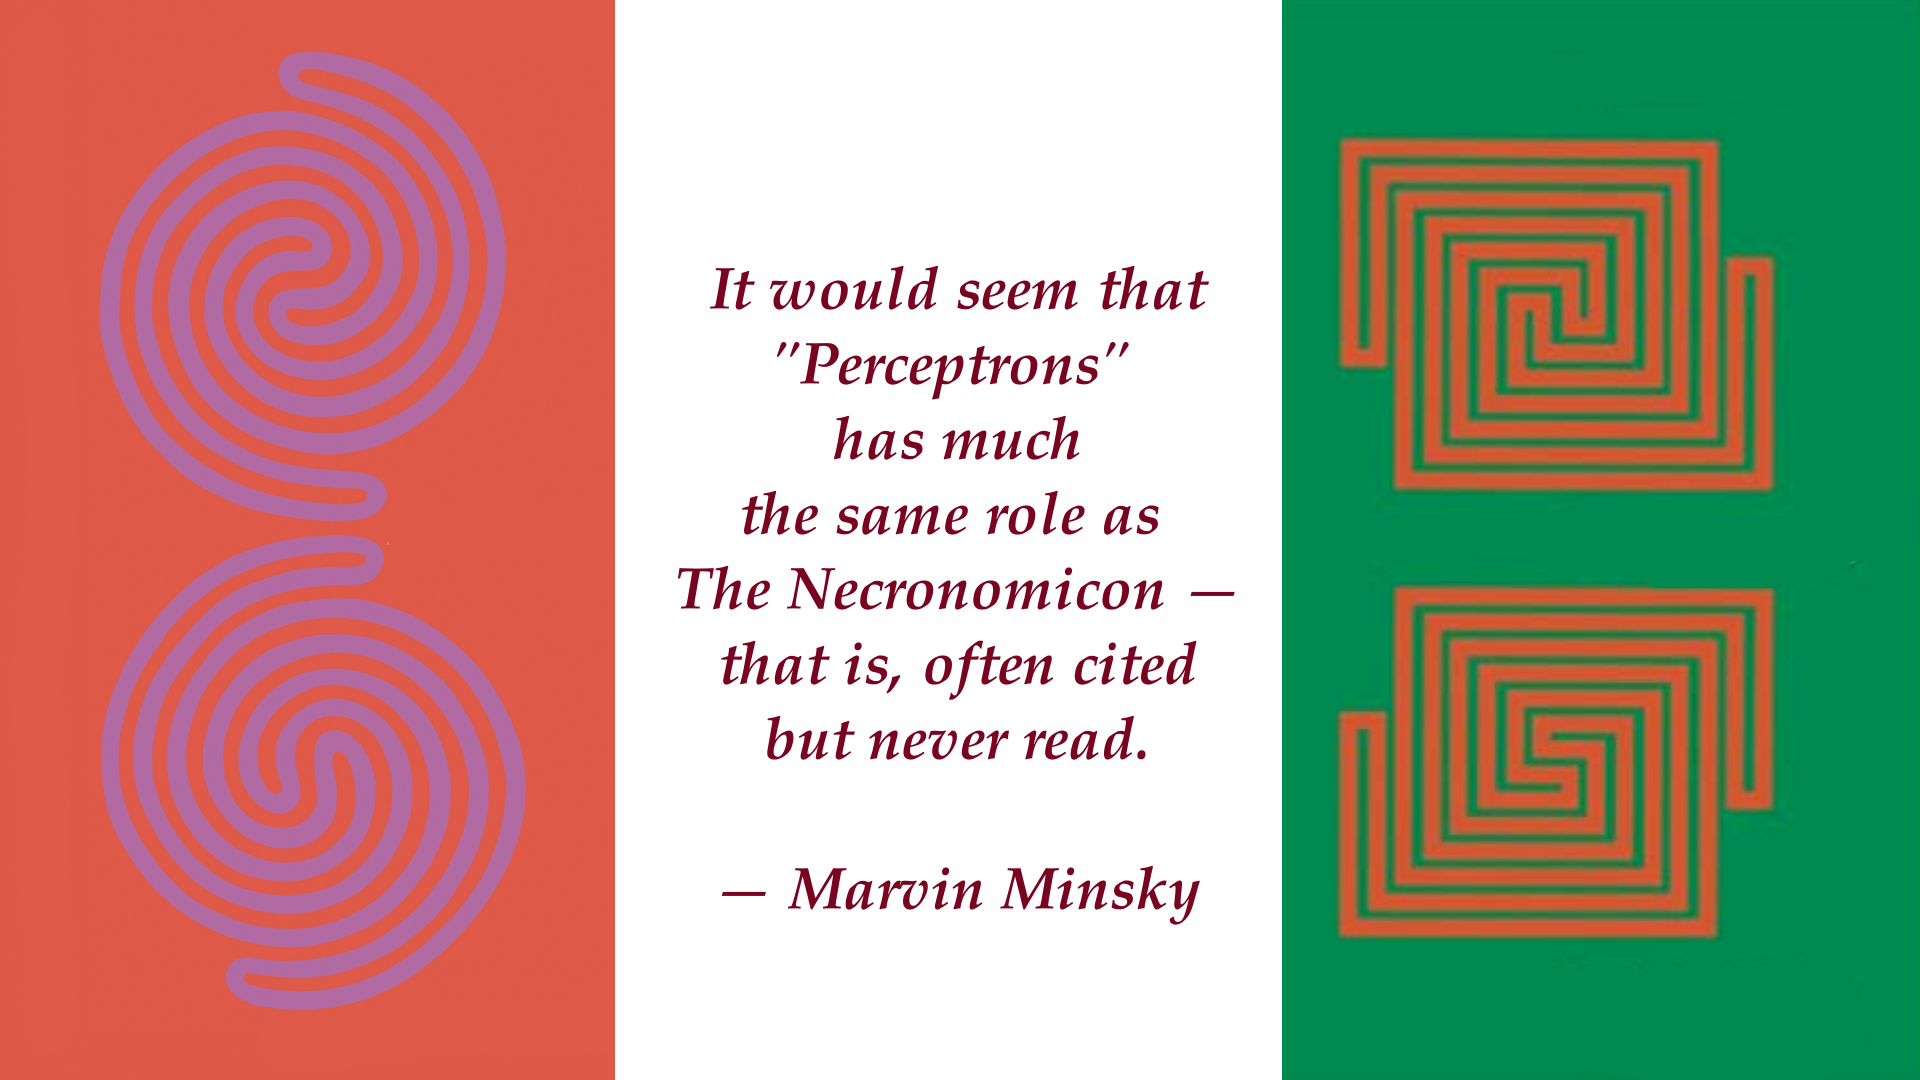
\includegraphics[width=1.3\textwidth]{figure/necronomicon_quote.png}}
    \end{figure}
\end{frame}
\begin{frame}
    \frametitle{XOR myth}
    The myth of XOR: Neural networks were abandoned after \textit{Perceptrons} (Minsky and Papert, 1969), which showed that a single-layered perceptron cannot learn the XOR function. It was revived in the 1980s after the development of multilayered perceptrons.

    \pause But...
    \begin{itemize}
        \item \textit{Obviously} XOR is impossible for single-layered perceptrons.
        \item McCulloch and Pitts (1943) already showed MLP as Turing-complete.
        \item Electric engineers were hand-designing MLP ("linear threshold logic") as Boolean logic modules.
        \item Rosenblatt, Widrow, SRI were all training MLP in the 1960s.
    \end{itemize}

    What is the real story?
\end{frame}

\begin{frame}
\frametitle{MLP fail}
Everyone failed to train MLP.

Rosenblatt had "back-propagating errors", continuous activation, and multiple trainable layers, but never gradient descent.

The other two groups did not fair any better.

\begin{displayquote}
We never succeeded in developing an algorithm for adapting both layers... Backprop to me is almost miraculous.

--- Bernard Widrow, 1994 interview. \cite[page 60--61]{rosenfeldTalkingNetsOral2000}
\end{displayquote}

\begin{displayquote}
I recall Charles Rosen, the leader of our group, sitting in his office with yellow quadrille tablets hand-simulating his ever-inventive schemes for making weight changes; none seemed to work out.

--- Nils Nilsson (of SRI) \cite[section 29.4]{nilssonQuestArtificialIntelligence2009}
\end{displayquote}

\end{frame}

\begin{frame}
\frametitle{Minsky \& Papert (1960s)}
\begin{itemize}
    \item Met in 1963. Started collaborating to dunk on large neural networks.
    \item Circulated their working notes at conferences.
    \item Also, on-stage debates. "Many remember as great spectator sport the quarrels Minsky and Rosenblatt had".
    \item Published their (in)famous book \textit{Perceptrons} in 1969.
\end{itemize}
\begin{figure}[t]
    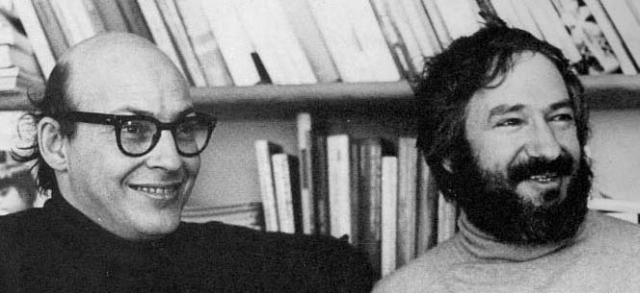
\includegraphics[width=\textwidth]{figure/Minsky_and_Papert.jpg}
    \centering
    \caption{Minsky (left) and Papert (right)}
\end{figure}

\end{frame}
    
\begin{frame}
\frametitle{Why Minsky?}

\begin{columns}
    \begin{column}{0.5\textwidth}
        Minsky: General algorithms never scale, only a Society of Mind Works
        \begin{figure}[t]
            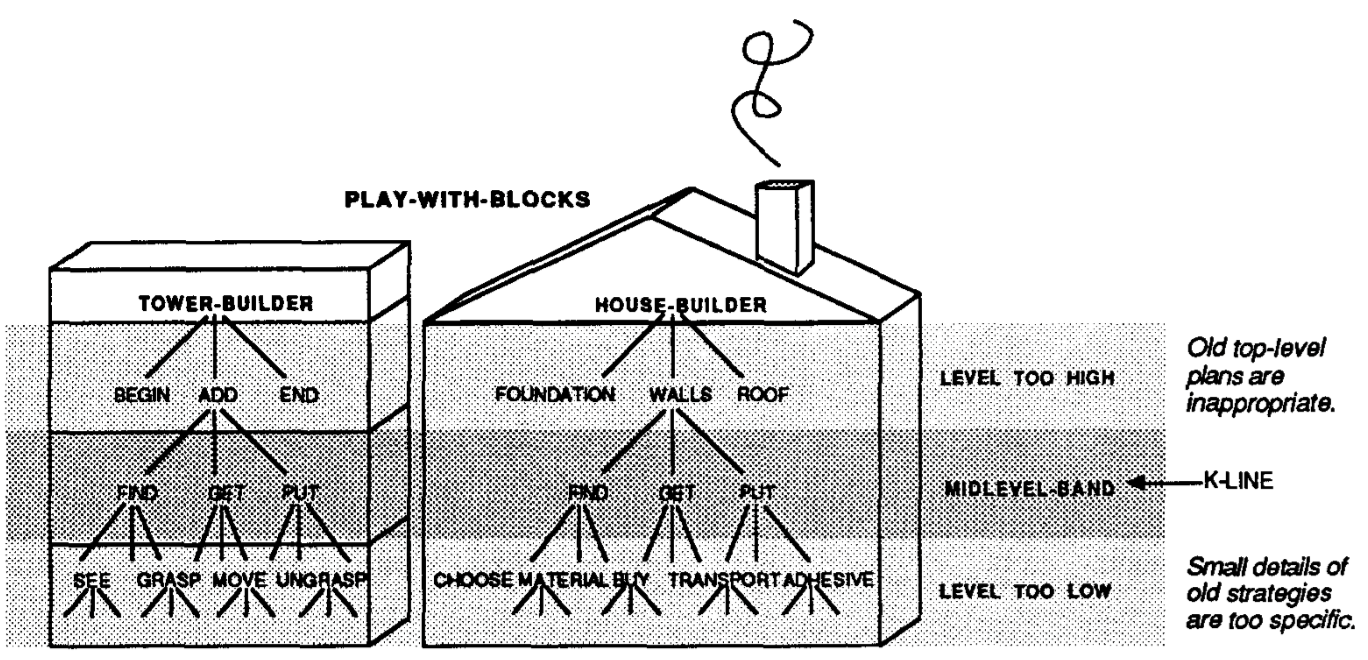
\includegraphics[width=\textwidth]{figure/Society_of_Mind.png}
            \centering
            \caption{Society of Mind \cite[section 8.6]{minskySocietyMind1988}}
        \end{figure}
    \end{column}
    
    \begin{column}{0.5\textwidth}
    \begin{displayquote}
        I had the naïve idea that if one could build a big enough network, with enough memory loops, it might get lucky ... either this was a bad idea or it would take thousands or millions of neurons to make it work, and I couldn't afford to try to build a machine like that.

        --- \cite{bernsteinMarvinMinskyVision1981}
    \end{displayquote}
    \end{column}
\end{columns}

\end{frame}

\begin{frame}
    \frametitle{Why Papert?}
    
    \begin{columns}
        \begin{column}{0.5\textwidth}
        \begin{displayquote}
            A new computer culture ... would require a new social construction of the computer, with a new set of intellectual and emotional values more like those applied to harpsichords than hammers. ... Epistemological pluralism is a necessary condition for a more inclusive computer culture.
    
            --- \cite{turkleEpistemologicalPluralismStyles1990}
        \end{displayquote}
        \end{column}    
        \begin{column}{0.5\textwidth}
            Papert: General algorithms are unjust and exclusionary to other ways of knowing. \textbf{Con}struction, not \textbf{In}struction
            \begin{figure}[t]
                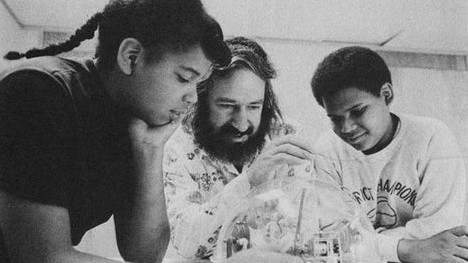
\includegraphics[width=\textwidth]{figure/Papert_with_children_and_robot.jpg}
                \centering
            \end{figure}
        \end{column}
    \end{columns}
\end{frame}

\begin{frame}
\frametitle{So what really caused the winter?}

\begin{itemize}
    \item Minsky and Papert's book: "our book put a stop to those" \cite{bernsteinMarvinMinskyVision1981}.
    \item Funding turned away from neural nets to the more symbolic methods.
    \item Lack of people
    \begin{itemize}
        \item McCulloch (1969), Pitts (1969), Rosenblatt (1971) died
        \item Widrow gave up MADALINE; focussed on ADALINE applications
        \item Ted Hoff went to Intel to invent microprocessor
        \item SRI turned to logical AI
    \end{itemize}
    \item No backprop.
\end{itemize}

\end{frame}

\begin{frame}
\frametitle{Why no backprop?}

\begin{itemize}
    \item Bad luck.
    \item Fear of local optima.
    \item Everyone "knew" that real neurons are binary, so artificial neurons must also be binary.
    \item They thought of machine learning as boolean function synthesis.
    \item ... but I don't know for sure. See my post for details.
\end{itemize}

\small{\url{https://yuxi-liu-wired.github.io/essays/posts/backstory-of-backpropagation/}}

\end{frame}

\begin{frame}
    \frametitle{Why the XOR myth?}
    Why do people keep teaching the XOR myth? My guess...
    \begin{itemize}
        \item Professors need to explain what happened during the 1970s in an introductory AI course.
        \item The actual XOR problem requires one to already understand perceptrons.
        \item The XOR problem is a convenient excuse.
        \item Thus -- the XOR myth!
    \end{itemize}
\end{frame}

\begin{frame}
    \frametitle{What is the actual XOR problem?}
    \only<1>{The XOR problem is real, despite the myth. See this flowchart...}
    
    \begin{figure}[t]
        \includegraphics<1>[width=\textwidth]{figure/XOR_problem_flowchart/1.png}
        \includegraphics<2>[width=\textwidth]{figure/XOR_problem_flowchart/2.png}
        \includegraphics<3>[width=\textwidth]{figure/XOR_problem_flowchart/3.png}
        \includegraphics<5>[width=\textwidth]{figure/XOR_problem_flowchart/5.png}
        \includegraphics<4>[width=\textwidth]{figure/XOR_problem_flowchart/4.png}
        \includegraphics<6>[width=\textwidth]{figure/XOR_problem_flowchart/6.png}
        \includegraphics<7>[width=\textwidth]{figure/XOR_problem_flowchart/7.png}
        \includegraphics<8>[width=\textwidth]{figure/XOR_problem_flowchart/8.png}
        \includegraphics<9>[width=\textwidth]{figure/XOR_problem_flowchart/9.png}
        \includegraphics<10>[width=\textwidth]{figure/XOR_problem_flowchart/10.png}
        \includegraphics<11>[width=\textwidth]{figure/XOR_problem_flowchart/11.png}
        \includegraphics<12>[width=\textwidth]{figure/XOR_problem_flowchart/12.png}
    \end{figure}
\end{frame}

\section{Neural Network Spring (1980s)}

\begin{frame}
    \centering{Neural Network Spring (1980s)}
    \begin{figure}[t]
        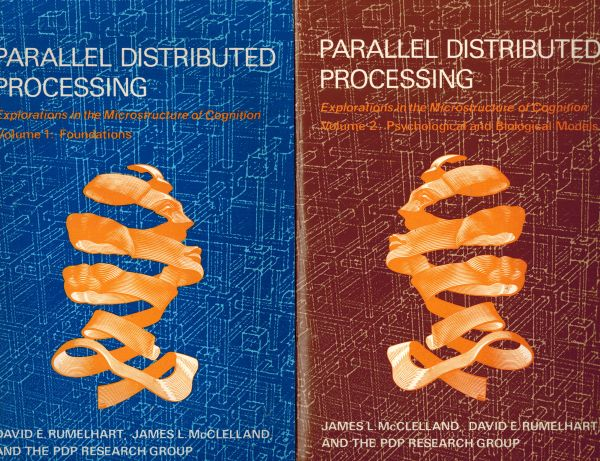
\includegraphics[width=\textwidth]{figure/PDP_book.jpg}
    \centering
    \end{figure}
\end{frame}

\begin{frame}
\frametitle{Spring has sprung (1980s)}

Why did neural networks emerge again in the 1980s?

\begin{columns}
\begin{column}{0.7\textwidth}
    \begin{itemize}
        \item Backprop developed multiple times, 1970s.
        \item But really hard to be known (just ask Paul Werbos).
        \item Also, widespread cheap compute (like PDP-11).
    \end{itemize}
\end{column}
\begin{column}{0.3\textwidth}
    \begin{figure}[t]
        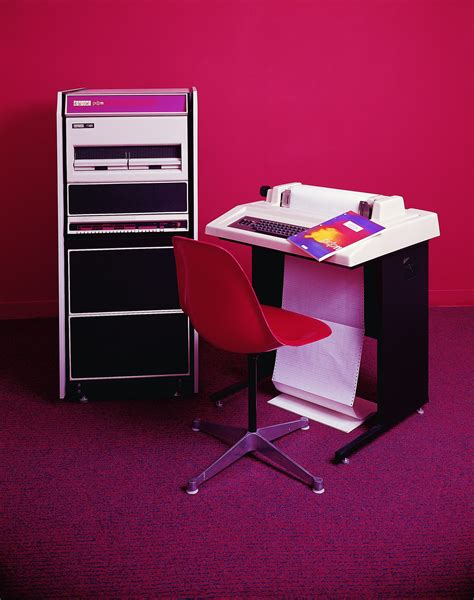
\includegraphics[width=\textwidth]{figure/PDP-11.png}
        \centering
        \caption{PDP-11 16-bit minicomputer (1970--1997)}
    \end{figure}
\end{column}
\end{columns}
\end{frame}

\begin{frame}
\frametitle{Paul Werbos}

\begin{itemize}
    \item Discovered backprop in 1972 during PhD, by mathematifying Freud's "psychic energy".
    \item Committee unsure of the math (or the Freud), "You've got to prove some theorems first." 
    \item Had to find a supporting advisor.
    \item Stephen Grossberg: "It's already been done before. Or else it's wrong. I'm not sure which of the two, but I know it's one of the two."
    \item Jerome Lettvin: "You're saying that there's motive and purpose in the human brain [like a Freudian, but] you cannot take an anthropomorphic view of the human brain."
    \item Marvin Minsky: "Everybody knows a neuron is a 1-0 spike generator... [Your model] is totally crazy."
\end{itemize}
\end{frame}

\begin{frame}
\frametitle{Paul Werbos}
\begin{itemize}
    \item So he simplified it down to piecewise linear activation.
    \item PhD committee: "too trivial to be worthy of a Harvard PhD".
    \item Lost funding; lived in the slums. "I remember getting the shakes from inadequate nutrition."
    \item Found a supporting advisor (Karl Deutsch, who wrote \textit{The Nerves of Government}).
    \item Finished PhD in 1974. Thesis contained backprop.
    \item A decade of misadventures working in the federal bureaucracy.
    \item Finally published backprop in 1982.
\end{itemize}
\end{frame}


\begin{frame}
\frametitle{Boltzmann machines}

\begin{itemize}
    \item Consider $n$ neurons connected by wires. Overall state of system is $X = (x_1, \dots, x_n)$.
    \item Energy of the system is $E(X)$.
    \item Probability of the system is $Pr(X) = \frac{e^{-\beta E(X)}}{\sum_{X'} e^{-\beta E(X')}}$.
    \item Many beautiful theorems. Physicists love this. 
\end{itemize}

\begin{figure}[t]
    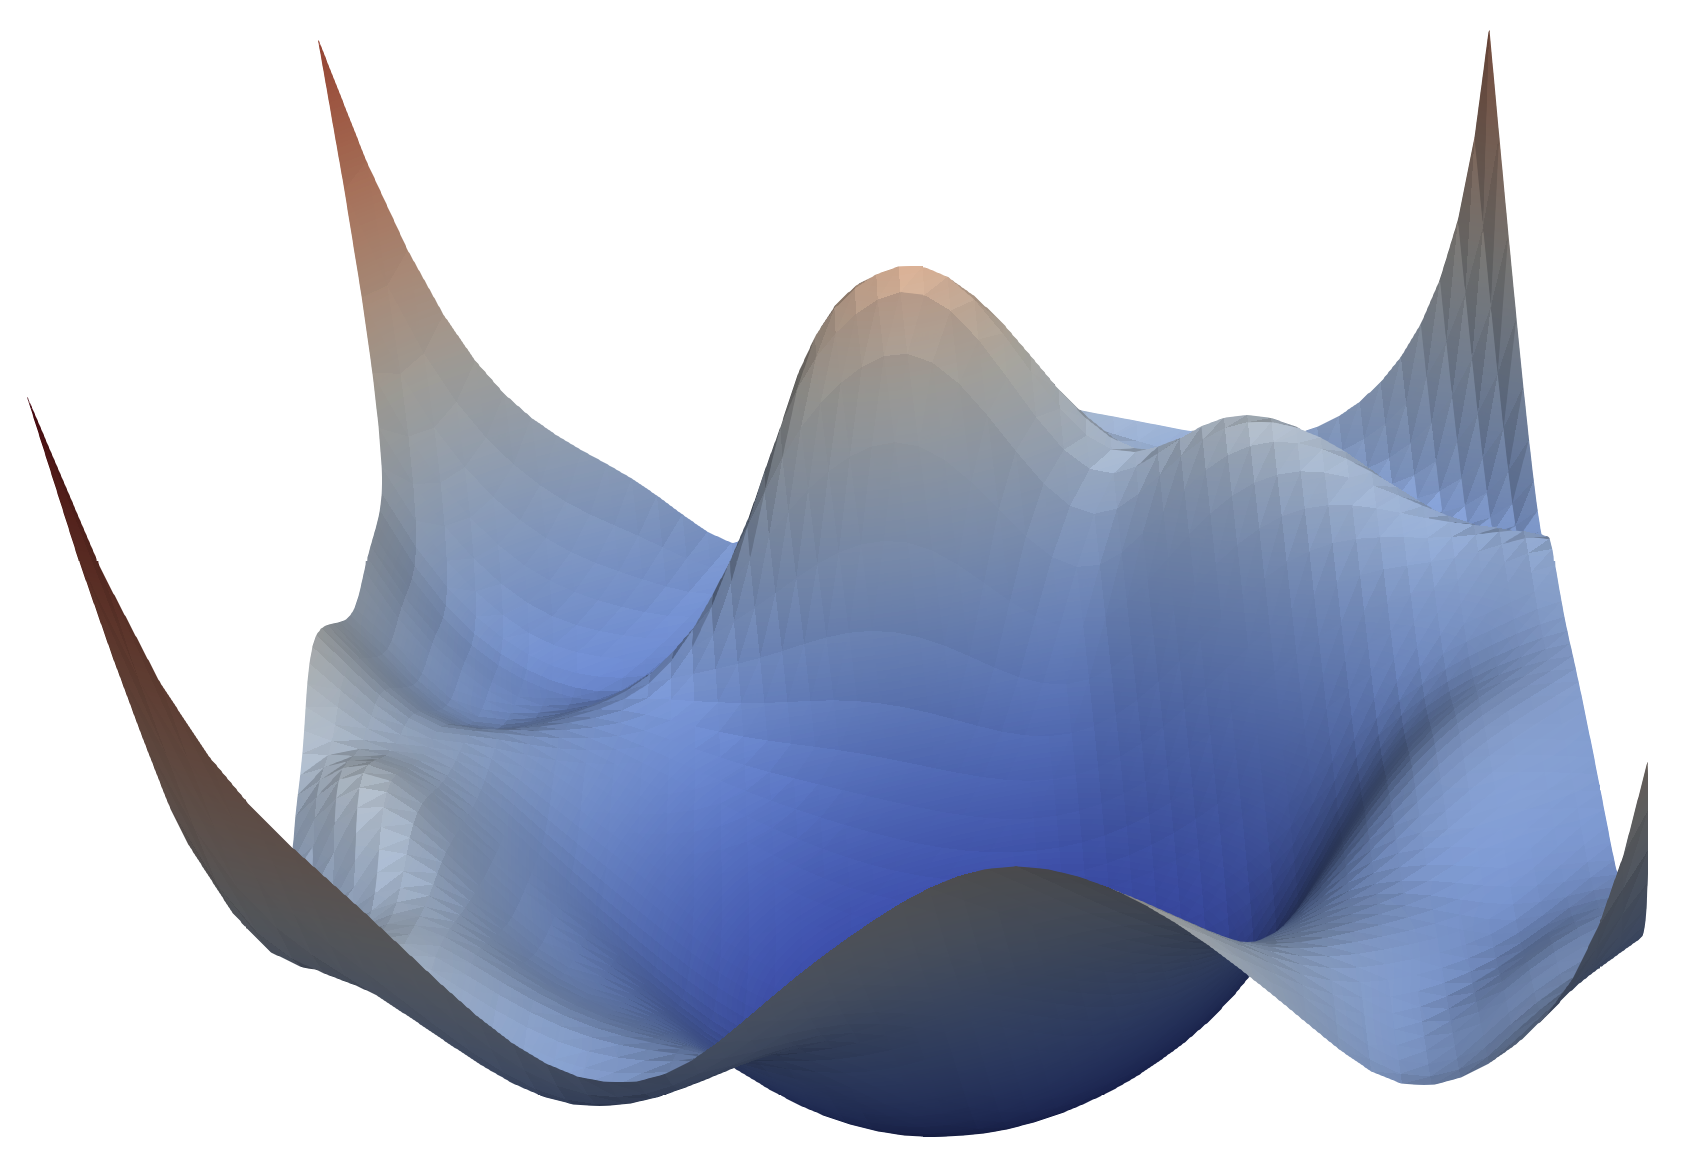
\includegraphics[width=\textwidth]{figure/energy_landscape.png}
    \centering
    \caption{Example energy landscape. \href{https://www.cs.umd.edu/~tomg/projects/landscapes/}{Source}}
\end{figure}

\end{frame}

\begin{frame}
\frametitle{Rumelhart and Hinton}

\begin{itemize}
    \item In 1982, David Rumelhart re-discovered backprop and told Geoffrey Hinton about it.
    \item Hinton resisted backprop for \textbf{3 whole years} before relenting.
    \item Hinton: "It couldn't break symmetry." -- Rumelhart: "Use noise."
    \item Hinton: "It gets stuck in local minima, unlike Boltzmann machine."
    \item Turns out Boltzmann machines also get stuck in local minima, oops.
    \item Boltzmann machines are beautiful, but they just don't work!
    \item Hinton's last resort: backpropagation (1985).
\end{itemize}
\end{frame}

\begin{frame}
\frametitle{Rumelhart and Hinton}

\begin{itemize}
    \item Asked his students: "Who wants to implement this?" 
    \item Students "thoroughly indoctrinated into Boltzmann machines" Refused to work on it, so Hinton programmed it himself.
    \item Tried it on an 8-3-8 autoencoder task. The weights looked weird.
    \begin{figure}[t]
        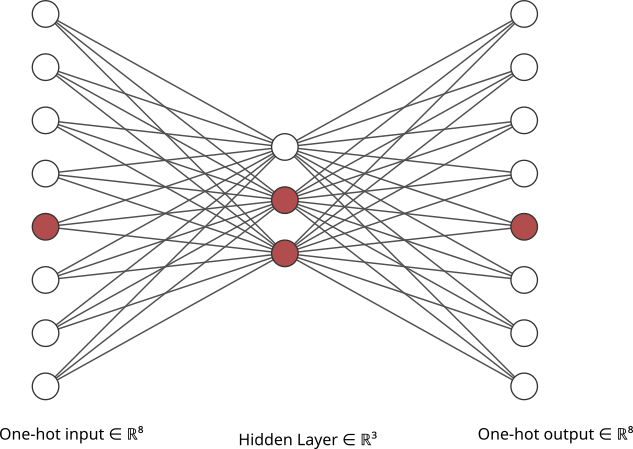
\includegraphics[width=0.5\textwidth]{figure/Hinton_8-3-8_autoencoder.png}
        \centering
    \end{figure}
    \item "Turns out backprop's not that good after all."...\pause wait, the loss is zero?!
    \item Published backprop (1985).
\end{itemize}
\end{frame}

\begin{frame}
\frametitle{Further controversies}
    
\begin{itemize}
    \item The \textit{Past-Tense Debate}, about whether statistical language models can truly learn linguistic rules.
    \item Started with a chapter in \textit{Parallel Distributed Processing} (1986); lasted well into 2000s. Died of exhaustion. \cite{seidenbergQuasiregularityItsDiscontents2014}
    \item Not very important now, but angered a lot of Chomskyan linguists.
    \item May be analogous to the modern debate about LLM?
\end{itemize}
\end{frame}

\begin{frame}
\frametitle{Further controversies}
    
\begin{itemize}
    \item Minsky and Papert re-published \textit{Perceptrons} (1988). Added over 40 pages of commentary re-rejecting large neural networks.
    \item Seems like people ignored Minsky and Papert this time.
\end{itemize}
\pause
\begin{figure}[t]
    \includegraphics<1>[width=\textwidth]{figure/XOR_problem_flowchart/13.png}
    \includegraphics<2>[width=\textwidth]{figure/XOR_problem_flowchart/14.png}
    \includegraphics<3>[width=\textwidth]{figure/XOR_problem_flowchart/15.png}
    \includegraphics<4>[width=\textwidth]{figure/XOR_problem_flowchart/16.png}
    \includegraphics<5>[width=\textwidth]{figure/XOR_problem_flowchart/17.png}
    \includegraphics<6>[width=\textwidth]{figure/XOR_problem_flowchart/18.png}
\end{figure}
\end{frame}
    
    
\section{Lessons}

\begin{frame}
\centering Some (bitter) lessons
\end{frame}
\begin{frame}
\frametitle{History is useless}
        
\begin{itemize}
    \item You can draw lessons from history, but everyone else also can draw the opposite ones.
    \item Use history to help you make history. Accuracy is overrated.
    \item History for history's sake is for old professors (that's Schmidhuber) and procrastinating PhD students (that's me).
\end{itemize}

\begin{displayquote}
We need it for life and action, not as a convenient way to avoid life and action... to value its study beyond a certain point mutilates and degrades life.

--- Nietzsche, \textit{On the Use and Abuse of History for Life}
\end{displayquote}
\end{frame}

\begin{frame}
\frametitle{Ideas can't be lost}
    
\begin{itemize}
    \item Ideas can't be lost.
    \item People will keep repeating the same ideas until it starts working, then it will not be lost again.
    \item Not the first inventor who gets the credit, but the last re-inventor.
    \item History is a cenotaph, useless for practitioners.
\end{itemize}

\begin{displayquote}
Those who cannot remember the past are condemned to repeat it.

--- George Santayana
\end{displayquote}
\end{frame}

\begin{frame}
    \frametitle{Ideas can't be lost}

    \begin{figure}[t]
        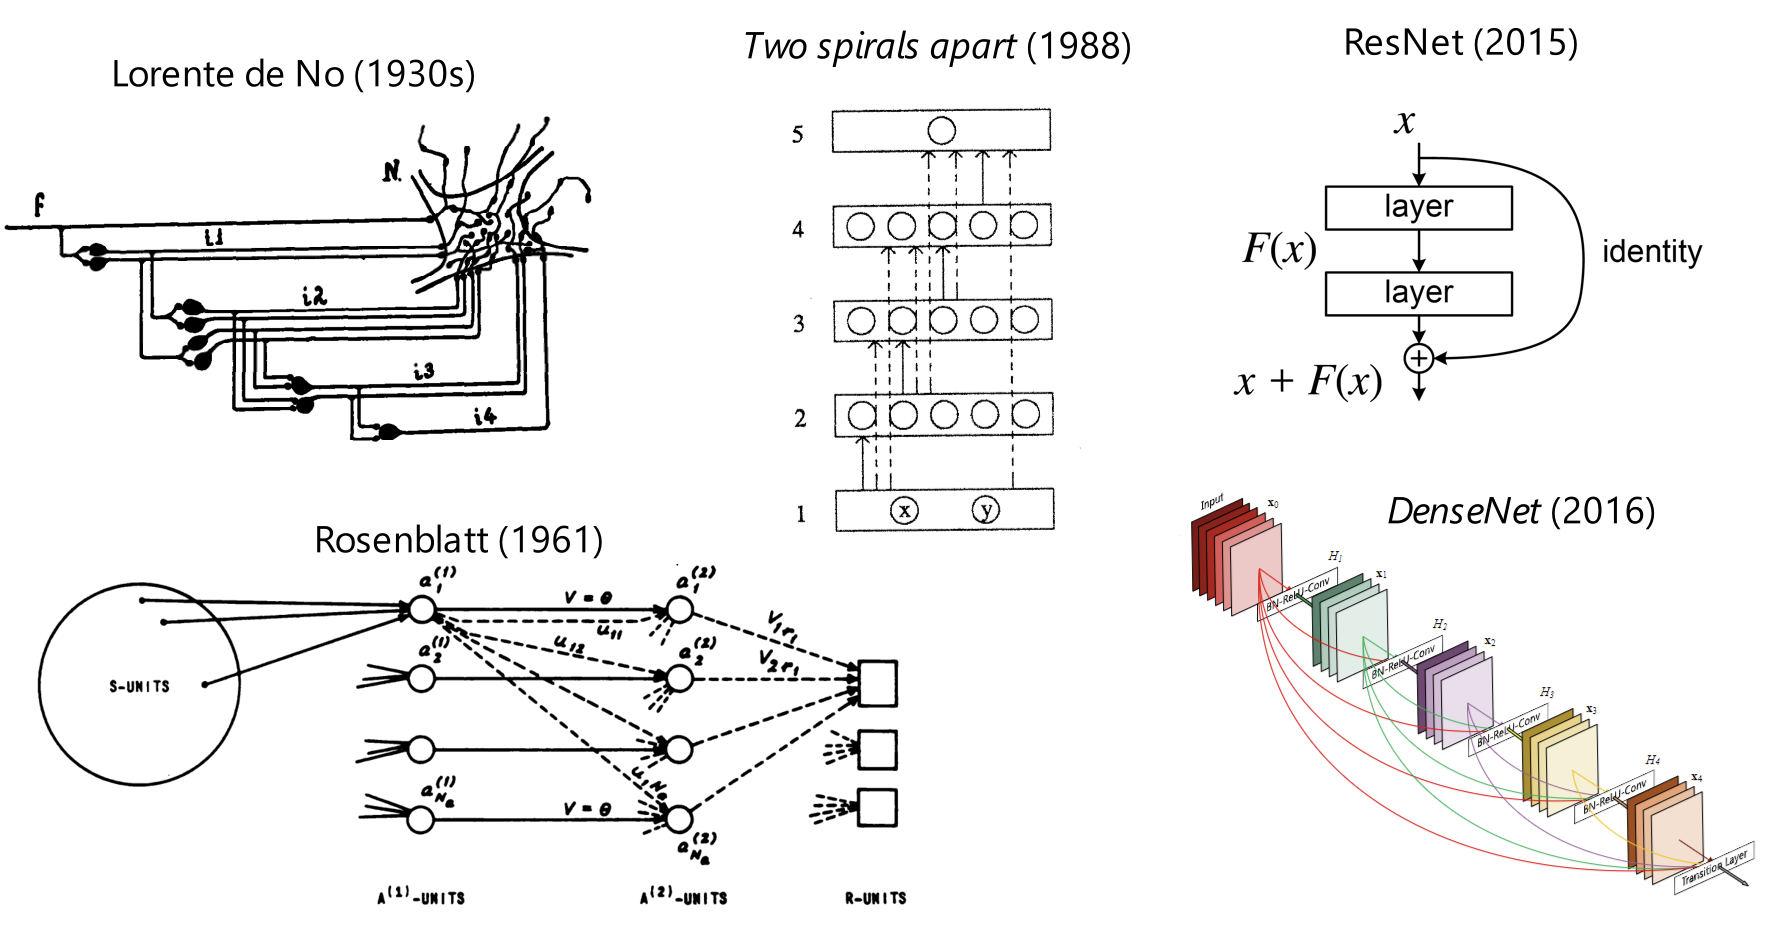
\includegraphics[width=\textwidth]{figure/ResNet_history.png}
        \centering
        \caption{Reinventions of the residual network.}
    \end{figure}
\end{frame}

\begin{frame}
    \frametitle{Ideas can't be lost}

    \begin{figure}[t]
        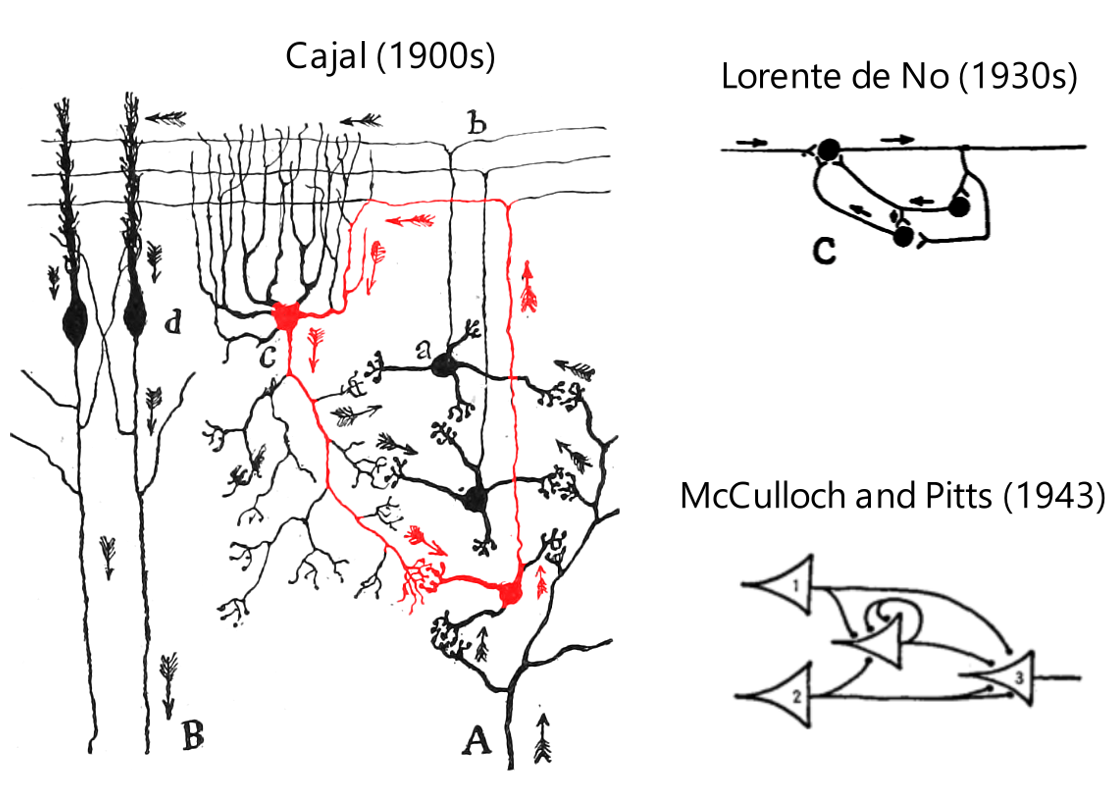
\includegraphics[width=0.8\textwidth]{figure/RNN_history.png}
        \centering
        \caption{Reinventions of the recurrent network.}
    \end{figure}
\end{frame}


\begin{frame}
    \frametitle{Compute matters more}
    \begin{itemize}
        \item For each elegant idea, there is an equal and opposite one.
        \item Benchmarks speak louder than ideas.
        \item Good ideas are patient seeds, waiting for the soil of compute. 
        \item cheap compute → cheap experiments → better ideas
    \end{itemize}
    \begin{displayquote}
        Which one helps, which doesn't help. Let's rip it out. Let's replace it with this... All of these components of the Transformer were the output of this extremely high-paced, iterative trial and error.  \cite{levyGoogleEmployeesInvented2024}
    \end{displayquote}
    \begin{displayquote}
        For months, they toyed with various ways to add more layers and still get accurate results. After a lot of trial and error, the researchers hit on a system they dubbed "deep residual networks". \cite{linnMicrosoftResearchersWin2015}
        \end{displayquote}
\end{frame}

\begin{frame}
    \frametitle{It just keeps bittering}

    \begin{itemize}
        \item Even with backprop, not much was possible in the 1970s. Ted Hoff was right to leave neural networks for Intel. But how many are like him?
        \item Minsky never accepted large neural networks.
        \begin{itemize}
            \item "We have not found (by thinking or by studying the literature) any other really interesting class of multilayered machine." (1969)
            \item "You're not working on the problem of general intelligence. You're just working on applications." (2006)
        \end{itemize}
        \item Noam Chomsky never accepted statistical language modeling.
        \begin{itemize}
            \item "the notion of 'probability of a sentence' is an entirely useless one, under any known interpretation of this term." (1969)
            \item "[Large language models] have achieved zero... GPT-4 will be exactly the same. It'll use even more energy and achieve exactly nothing, for the same reasons. So there's nothing to discuss." (2022)
        \end{itemize}
    \end{itemize}
\end{frame}

\begin{frame}
    \frametitle{It just keeps bittering}
    \begin{itemize}
        \item Even Geoffrey Hinton remained unhappy about backprop.
        \item "I was always a bit disappointed. I mean, intellectually, backpropagation wasn't nearly as satisfying as Boltzmann machines. It's not just because I didn't think of it. I think it's because it didn't have the nice probabilistic interpretation." (1995)
        \item Also he was doing Deep Belief Networks (multilayered Boltzmann machines) up until 2009.
        \item And so, the bitter lesson continues...
    \end{itemize}
\end{frame}


\begin{frame}
    \frametitle{Further reading}
    \begin{itemize}
        \item \url{https://yuxi-liu-wired.github.io/essays/posts/backstory-of-backpropagation/}
        \item \url{https://yuxi-liu-wired.github.io/essays/posts/reading-perceptron-book/}
        \item \url{https://yuxi-liu-wired.github.io/essays/posts/perceptron-controversy/}
        \item \url{https://yuxi-liu-wired.github.io/sketches/posts/history-neural-networks-talk-notes/}
    \end{itemize}
\end{frame}
\bibliographystyle{apalike}
\bibliography{references}
\end{document}